\documentclass[withoutpreface,bwprint]{cumcmthesis} %去掉封面与编号页，电子版提交的时候使用。

\usepackage[style=authoryear]{biblatex} % 作者-年份样式
\usepackage{pdfpages}
\usepackage[UTF8]{ctex} % 中文支持
\addbibresource{refs.bib} % 指定.bib文件

\usepackage{setspace}
\renewcommand{\arraystretch}{1.5} % 默认1.0，增大值增加行高

\usepackage{cleveref}
\usepackage{hyperref}

\usepackage[framemethod=TikZ]{mdframed}
\usepackage{tcolorbox} % 替代mdframed，更好的边框支持
\usepackage{url}   % 网页链接
\usepackage{subcaption} % 子标题
\title{\zihao{2}{ComplierMind: LLM+编译原理助学平台}}


\tcbset{
    mydashedbox/.style={
        colback=white,
        sharp corners,
        left=0.2pt,        % 左侧内边距极小
        right=0.2pt,       % 右侧内边距极小
        top=0.2pt,         % 顶部内边距极小
        bottom=0.2pt,      % 底部内边距极小
        boxrule=1.2pt
    }
}

% 更灵活的环境定义
\newenvironment{imageandboxflex}[2][0.4]{% 可选参数为图片宽度比例，默认0.4
    \begin{minipage}[t]{#1\textwidth}
        \vspace{0pt} % 关键技巧：实现顶部对齐
        \centering
        \includegraphics[width=\linewidth]{#2}
    \end{minipage}\hspace{0pt}% <-- 添加 \hspace{0pt}
    % \hfill
    \begin{minipage}[t]{\dimexpr0.9\textwidth-#1\textwidth\relax}
        \vspace{5pt} % 关键技巧：实现顶部对齐
}{%
    \end{minipage}\hspace{0pt}% <-- 添加 \hspace{0pt}
}

% 更灵活的环境定义
\newenvironment{withimageandboxflex}[2][0.4]{% 可选参数为图片宽度比例，默认0.4
    \begin{minipage}[t]{#1\textwidth}
        \vspace{0pt} % 关键技巧：实现顶部对齐
        \centering
        \includegraphics[width=\linewidth]{#2}
    \end{minipage}\hspace{0pt}% <-- 添加 \hspace{0pt}
    \hfill
    \begin{minipage}[t]{\dimexpr0.9\textwidth-#1\textwidth\relax}
        \vspace{-3pt} % 关键技巧：实现顶部对齐
}{%
    \end{minipage}\hspace{0pt}% <-- 添加 \hspace{0pt}
}



\begin{document}

\includepdf[pages={1-2}]{al.pdf}

 \maketitle

 \begin{abstract}

本项目以农大东校区为地点，使用C++为主要算法语言，开发
一个PHP\&JavaScrip架构的网页系统。
融入地图经纬度、搜索定位、两点间路径规划(DFS，Floyd, Yens)、
多景点路径规划、最优景点推荐机制。
提出了带边表，Floyd表压缩算法，
特殊目标规划模型等创新点。同时也应用蚁群算法合理解决问题。

\textbf{关键词}：中国农业大学，导览，推荐，图论，带边表，Floyd表压缩算法，蚁群算法，Floyd算法，暴力TSP，
多目标规划，php\&JavaScrip\&C++架构，leaflet调用

 \end{abstract}




\section{问题描述}

\subsection{问题描述}

我们的目标是设计一个校园导览系统，为来访的客人提供导游服务。

目标点是为客人提供较好的\textbf{导游服务}。其核心是路径规划和景点推荐两个
主要功能。优化方向也是景点推荐算法，用户画像获取，景点分类与推荐等几个方向。
基于算法课的方向，我们的核心是以图论算法的应用为主，路径规划的算法求解与比较为基础，
景点的推荐与用户画像为进阶，完成一个基本的导览系统。



\subsection{基本要求}

基本要求包括不少于十个的校园景点数，完整的图论展现形式，为客人提供图中任意景点的
查询操作。为客人提供任意节点间的问路查询，即最短路径。

整体要求实际上就是深入挖掘图论的基本算法，以景点规划为常见案例，考量经典的路径规划、
图论搜索、最优查找、合理推荐的方面。在此基础上进行最短路径规划问题，旅行商问题，
任意多景点规划问题，观光者问题的图论求解。



\subsubsection{实现目标}
我们的实现目标是实现一个应用舒适，功能齐全，具有一定推荐功能的导览系统。

在\textbf{形式展示}上，我们的目标是一个网页端的界面和四个主要的界面功能。
通过这个导览网页来满足基本导游系统的需要。

在\textbf{算法呈现}上，我们的目标是通过导览系统为载体，深入研究图论相关
的各类算法技术。最短路径，TSP，匹配算法，推荐算法\dots

在\textbf{对象选择}上，我们以农大的13个景点为预设载体，探究在这3个景点之上
的游览、推荐需求，进行实现。


\subsubsection{数据输入}
\noindent 具体的数据输入如下所示:
\[
\begin{cases}
    \text{13个结构体，景点的经纬度以及基本相关信息输入。}\\
    \text{13*13的邻接矩阵，我们采用的是边权为路径距离(非
    直线路径距离，实际距离的矩阵模式)。}\\
    \text{5维的速度向量，不同类型人群的步行速度} \\
    \text{13*5的时间矩阵，不同类型人群在不同景点的停留时间矩阵} \\
    \text{13*5的效益矩阵，不同类型人群对不同景点的效益感知矩阵}
\end{cases}
\]

\subsubsection{数据输出}
\noindent 具体的数据输出如下所示：
\[
\begin{cases}
    \text{所有点的经纬度点位信息以及相关的附注信息汇总}\\
    \text{整张图中的所有两点间的直接相连的一次路径}\\
    \text{任意两点的一条最短路径，以及任意两点间的TopK条最短路径，
    以及任意两点间的全部路径}\\
    \text{至少经过任意多景点的最优游览路径}\\
    \text{任意可选人群在给定时间下推荐游览的路径}
\end{cases}
\]

\subsection{初步思路}

\subsubsection{基本假设}

\begin{itemize}
    \item 假设系统中\textbf{景点}与\textbf{路点}
    是等价的（注：经过分析我们认为在成熟的导航系统，比如
    高德，会以\textbf{路口}为路点，进行路径规划，
    我们采用简化模型，将景点直接视为路点。）
    \item 在游玩路径推荐部分，假设不同人群的步行速度为
    一个\textbf{定值}，同时不同的人群内部效益\textbf{一致}。同时归属多个人群的人直接对步行速度、
    停留时间和景点效益取\textbf{多个人群的平均值}。
\end{itemize}

\subsubsection{基本思路}

初步思路是首先确定\textbf{系统内容和边界}，
以图论为核心，完成导览和推荐系统的工作，
目前不做生态圈系统拓展的相关功能。
同时导览系统的形式以二维地图
导览为主，不添加AR/VR/ER元素。
同时限制点为13个校内景点。


其次，在PHP+JavaScrip+exe(C++)的经典架构上，
引用leaflet，导入从高德上下载的瓦片，再进行
13个顶点的经纬度查询与标注。

然后，绘制13个顶点的实际图示和查询绘制其中边。
接着，进行初始界面设计和基本输入存储设计。
并采用leaflet的集成化工具将输入数据呈现处理。

随之，我们开始逐项完成下面的规划和推荐的两大部分
功能。
对于C++代码与php的集成，我们采用基础的exe命令行交互模式完成。
从而完成整个项目。



\begin{figure}[!h]
\centering
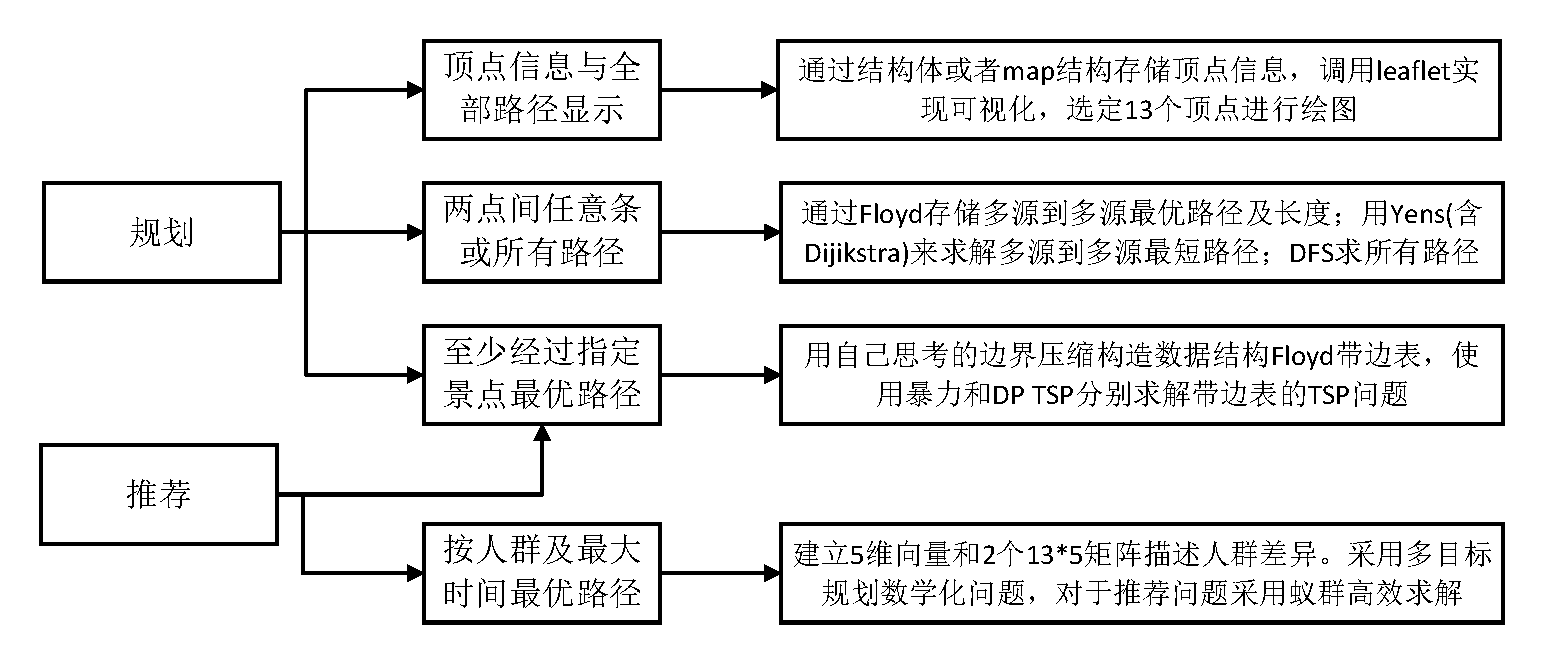
\includegraphics[width=1.0\textwidth]{figures/流程图.pdf}
\caption{整体功能设计流程图}\label{fig:f1}
\end{figure}


\section{算法与工程内容汇总}
具体结构见附录A，下面着重
讲解我个人负责的工程内容和数据结构与算法。其中
页面可视化主要由我来负责，数据搜集和数据模型编写
队友负责，算法我们分别做。

\subsection{主页面和路径展示页面，用于展示各点信息和实际图点位}

\begin{figure}[!h]
\centering
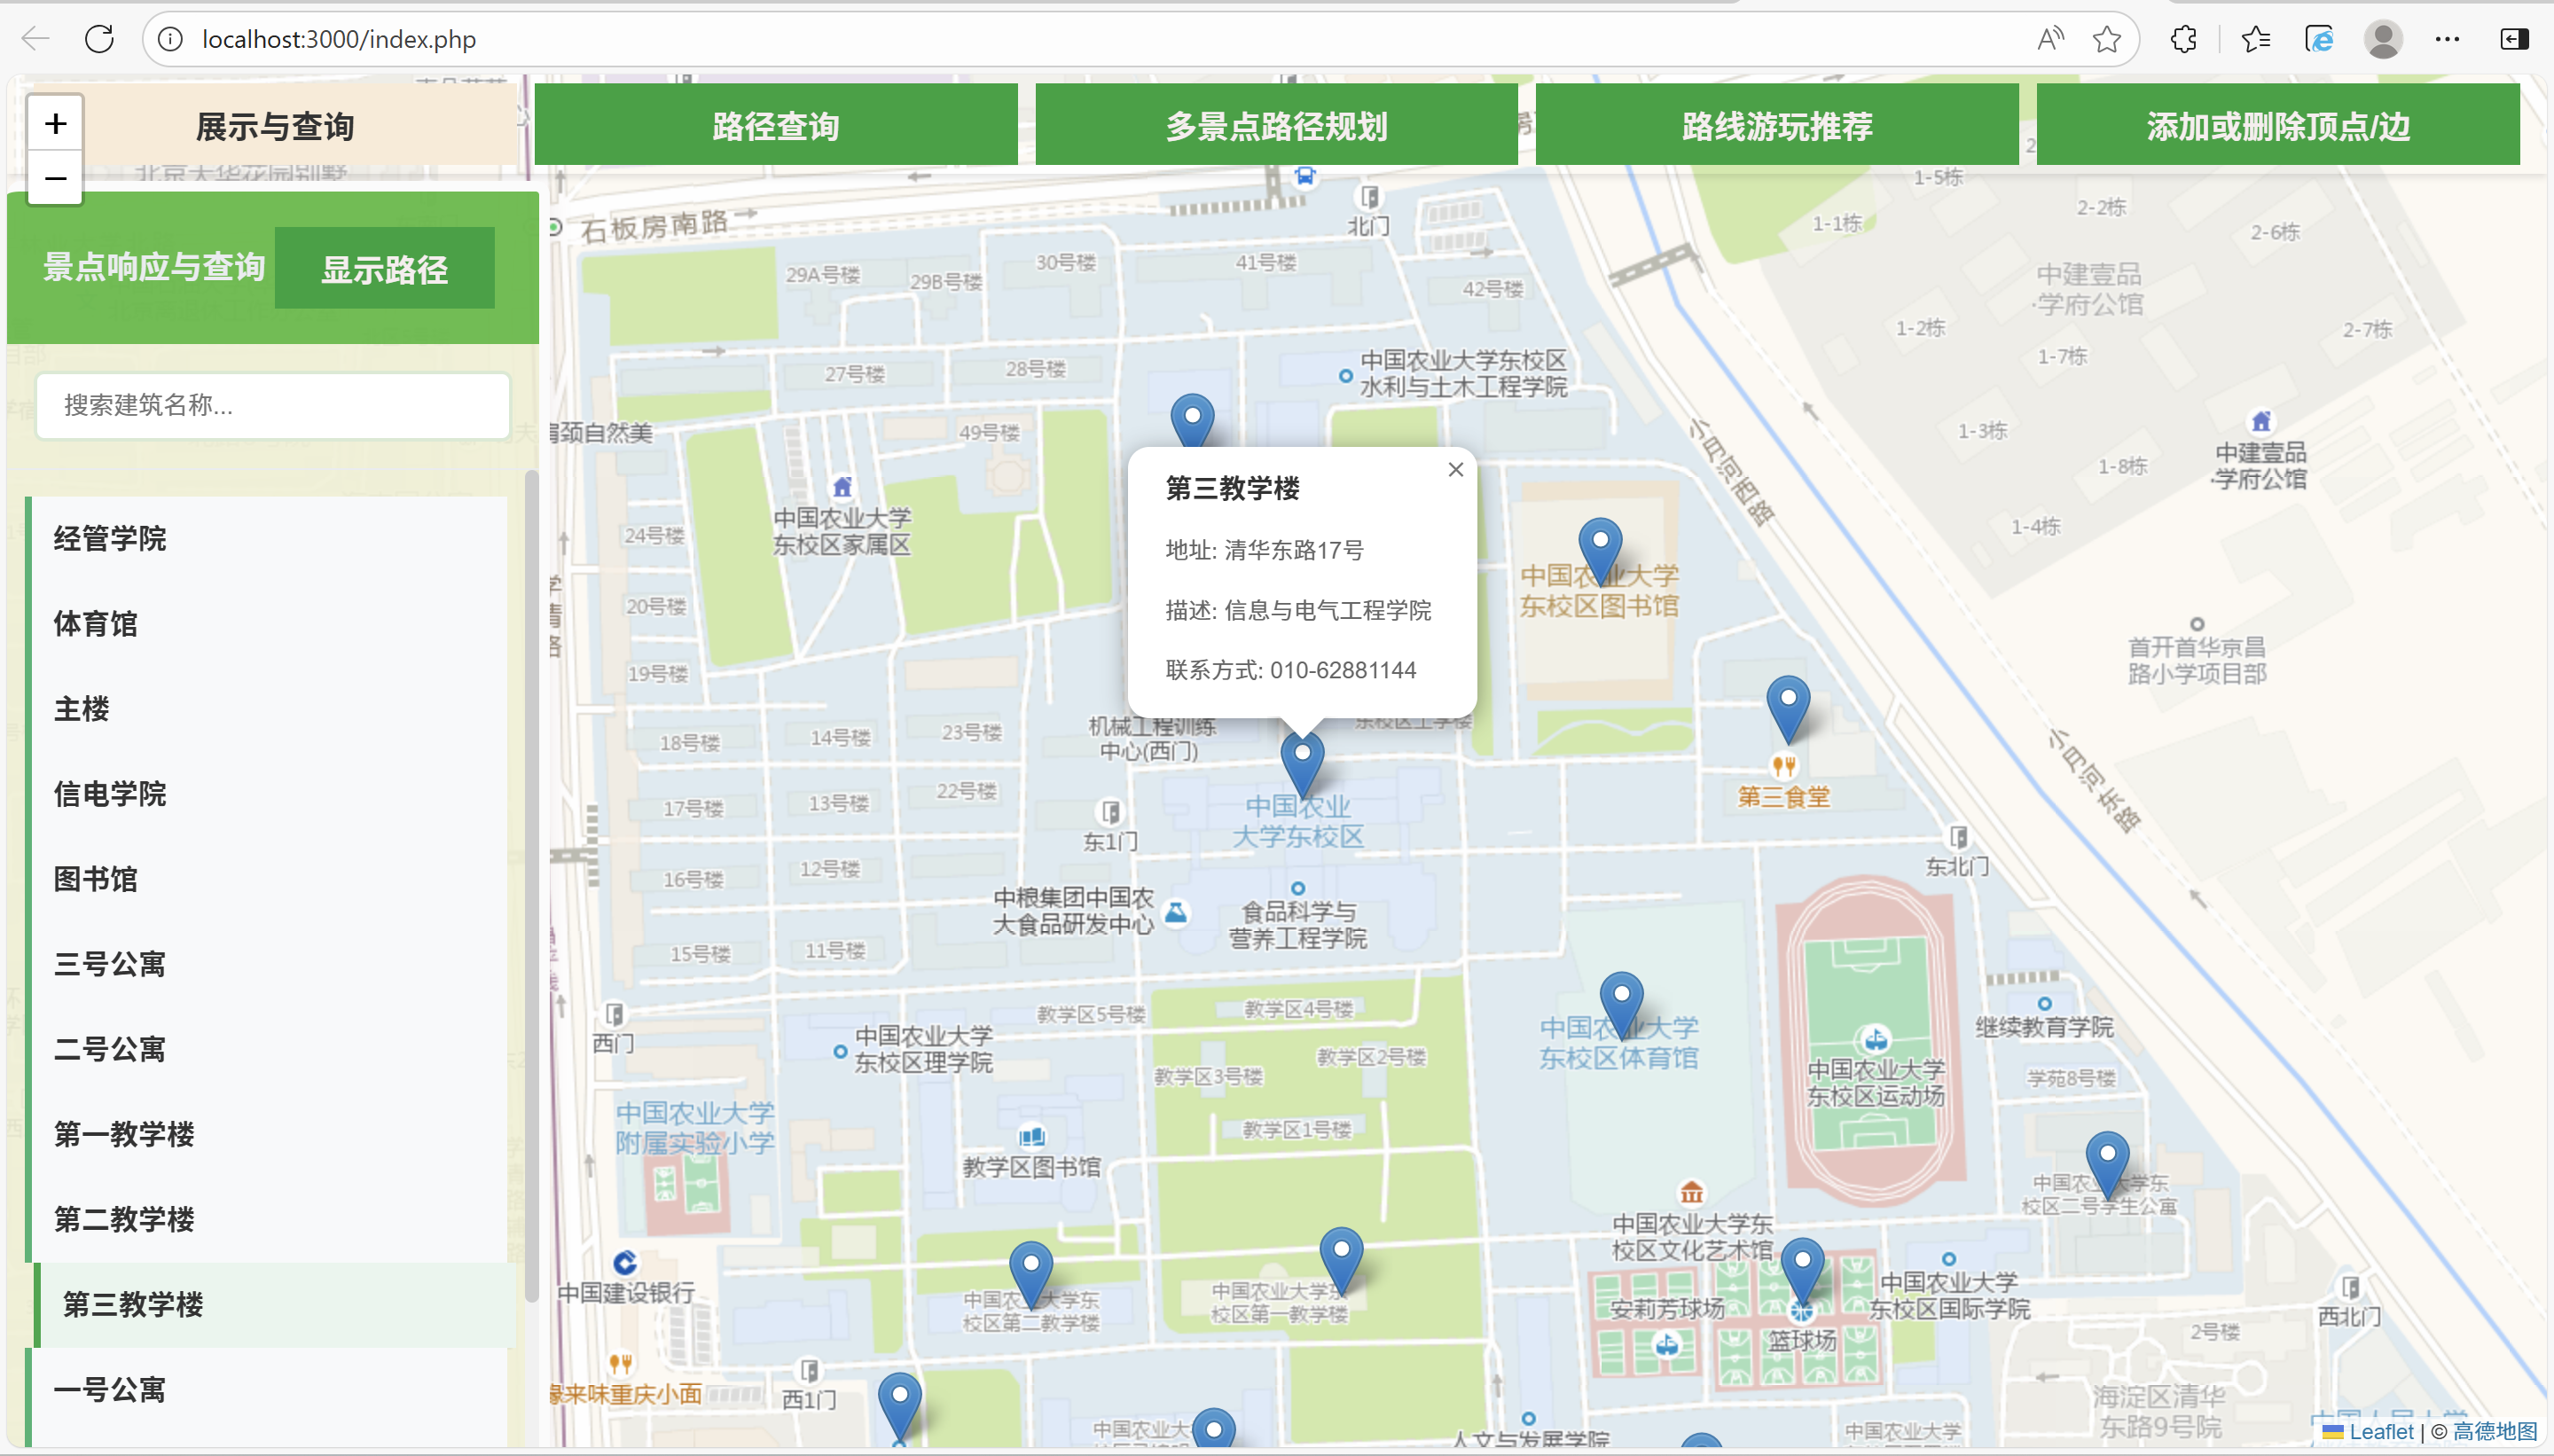
\includegraphics[width=0.9\textwidth]{figures/index.png}
\caption{主界面展示图}\label{fig:f2}
\end{figure}

\begin{figure}[!h]
\centering
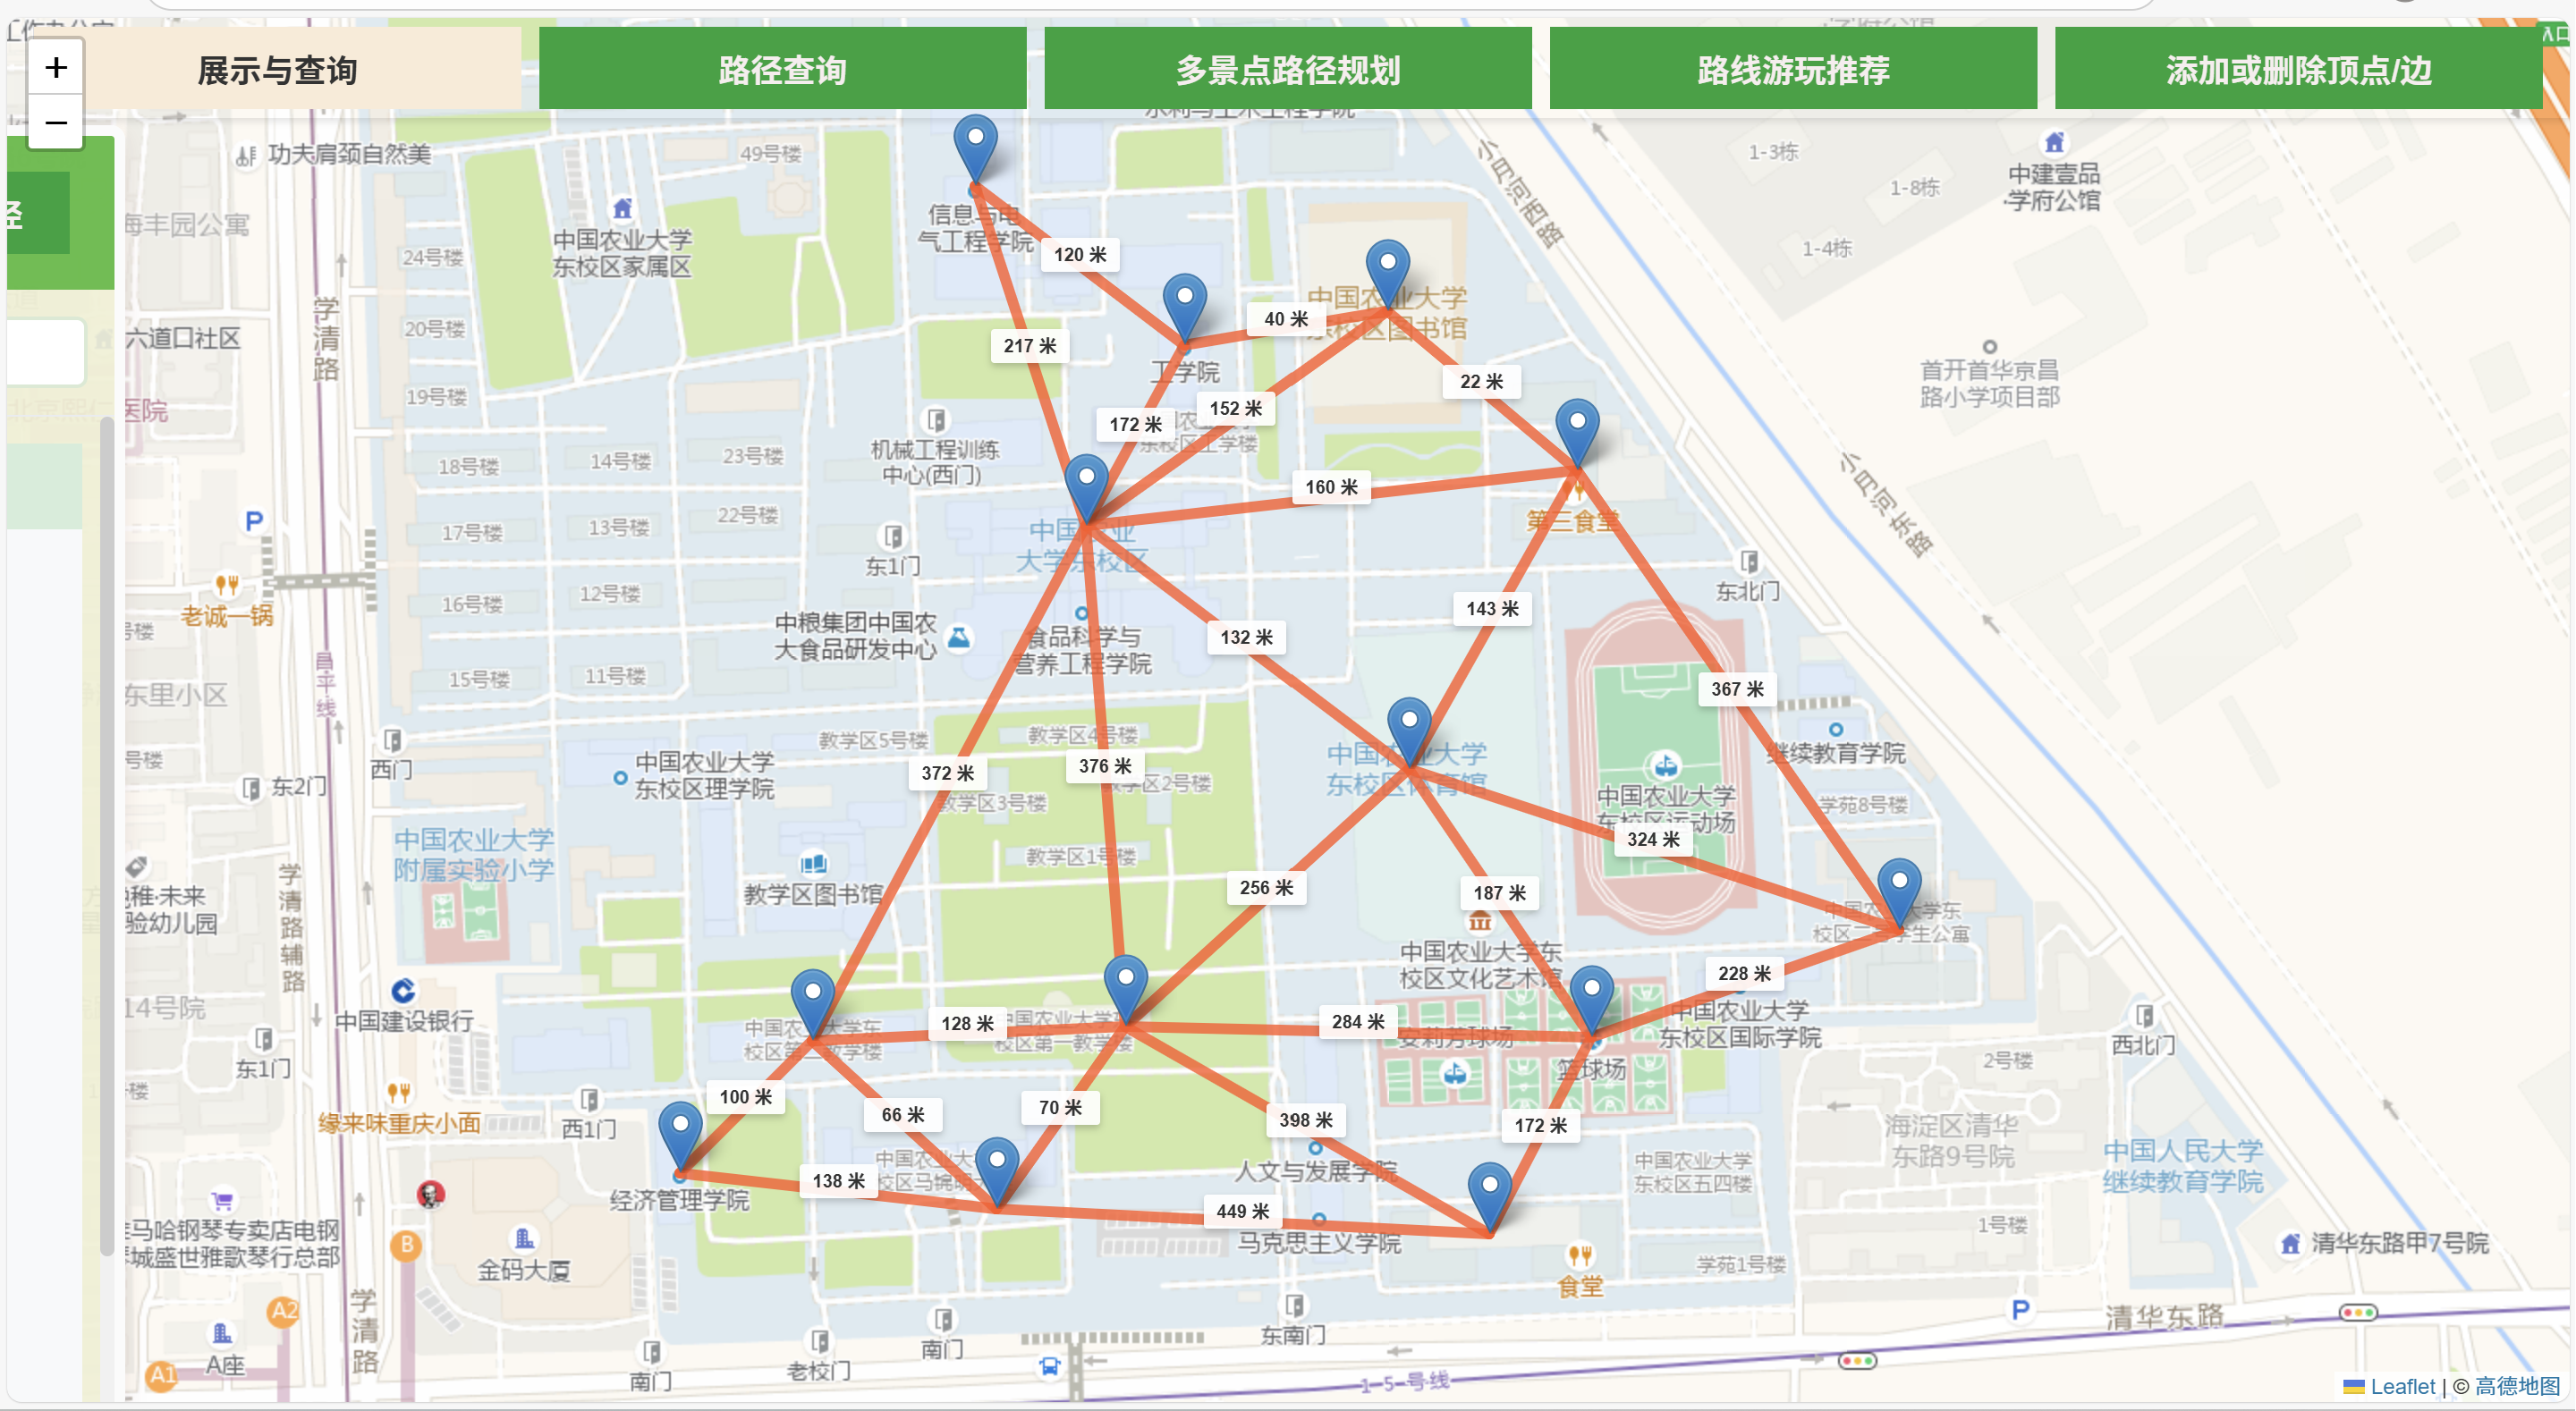
\includegraphics[width=0.9\textwidth]{figures/1.png}
\caption{所有路径展示图}\label{fig:f3}
\end{figure}

其中我个人负责web网页的可视化，输入输出和显示，
队友负责搜集数据，对道路网络进行剪枝处理。

上述的图模式是更新版的结果，
在开始，我们认为首先发现任意景点之间实际上都是互通的
实际上他们之间的矩阵应该是一个13*13的满矩阵。做出图如下：


\begin{imageandboxflex}[0.49]{figures/13个节点图.pdf}
    \begin{tcolorbox}[mydashedbox]
    \noindent \hspace{2em} 左图是我们的13个节点彼此
    任意相连的满邻接矩阵图示，含有78条边结构，非常复杂
    而不简洁。（左图没有将0 \~ 12号节点放在对应的位置，
    仅用于展示图的拓扑连接关系）在推进过程中，我们发现
    造成这样的原因是由于\textbf{没有考虑真实路径的关系}。
\end{tcolorbox}
\end{imageandboxflex}
\vspace{2em}

实际上上面的图中很多相连的景点实际上是
部分复用了同一条路径。
分析原因：实际上是由于在这个图中我们\textbf{把景点直接当作
了路点}，但是没有进行特殊处理导致的。

这里的特殊处理有两种：

1.进行剪枝（剪掉所有两边之和小于或等于第三边的边）。
因为实际上\textbf{真实路径的关系}已经含在两边等于或小于第三边的这个
数学信息中了。

2.根据实际路径关系进行路点分析（实际上也有一定
的剪枝处理）。

因为上述问题的成因来源于路径信息的缺失，这样获得的数据形式应该是
路点，而不是景点。当我们做出景点等效路点的假设时，
必须采取上面的特殊处理。

这里我们\textbf{考虑一个可能会可以深入探讨的算法}，对应方法1，
直接进行剪枝处理。利用计算机可能可以实现算法。
然后我们由于时间限制，
暂且还是采用经典的方法2重画了抽象出来的景点图，
就是现在系统中展示出来的图。


\subsection{路径查询页面}

其中这里有三个功能，当k=1时显示1条路径，
采用\textbf{Floyd算法}生成一张表（在现实应用中
在每次增删节点或修改节点时重新生成一次，
每次读表可以节省时间开销）；
当k$\ge$2时显示k条路径(直至显示全部为止)，
采用\textbf{Yens算法}来生成；
当k=dfs时显示全部路径，采用\textbf{深度优先搜索}来
进行穷搜(注意这里节点数少，是可以实现的)。

然后这一部分第一个k=1的\textbf{Floyd算法}是我负责的，
图形化展示(php和exe交互)是我负责的。

\subsubsection{图形化展示Floyd算法}

\begin{figure}[!h]
\centering
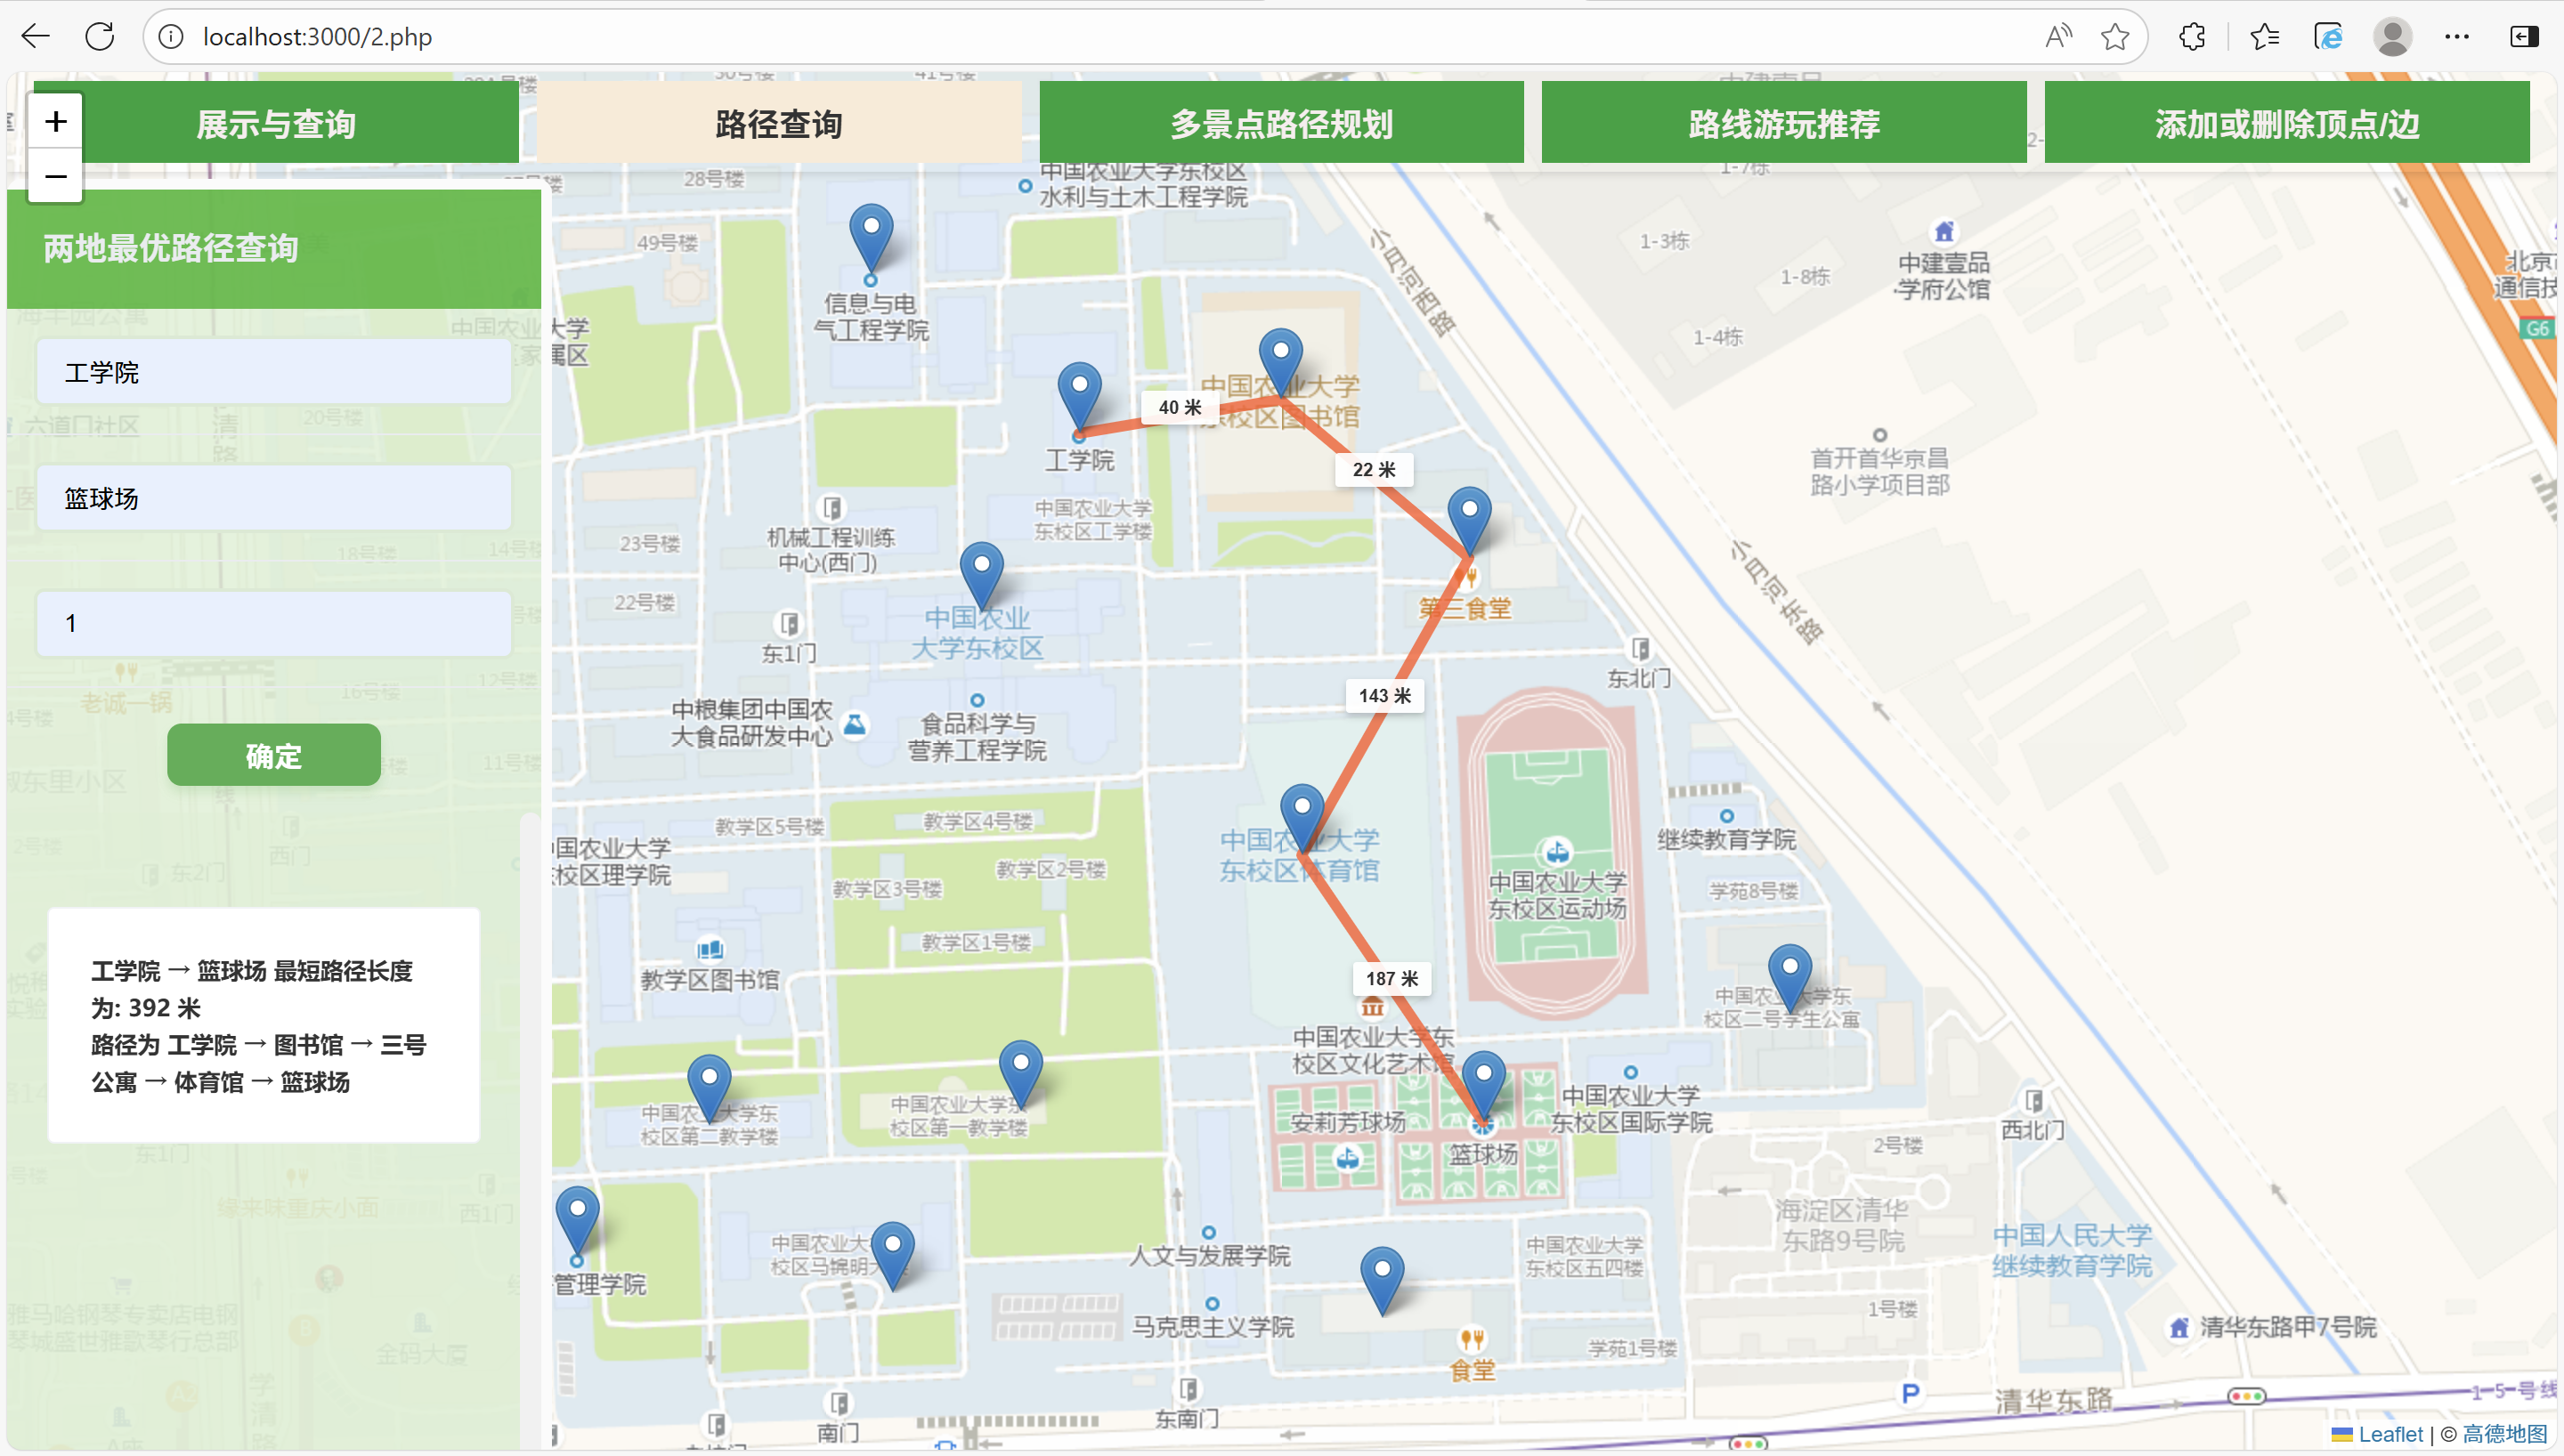
\includegraphics[width=0.9\textwidth]{figures/2.png}
\caption{Floyd最短路径应用}\label{fig:f4}
\end{figure}

\subsubsection{Floyd算法的内容与算法分析}
实际上Floyd算法是在生成两个矩阵，
一个是最短路径长度矩阵lens，
一个是路径矩阵paths。
其本质是一个可优化空间的动态规划。
对于最短路径长度状态方程如下：
\begin{equation}
    dp[k][i][j] = min\{dp[k-1][i][j], dp[k-1][i][k-1]+dp[k-1][k-1][j]\}
\end{equation}

由于这个动态规划每次只需要前一次的最短长度矩阵，
是一个特殊的三维动态规划，所以可以只用一个lens
矩阵来进行存储。

对这个状态转移方程进行解释即为
第k次尝试缩短时的从i到j的路径，要么是第k-1得到的结果，
要么是从i到k-1，再从k-1到j之和。

上面是lens的状态方程，而paths矩阵也随时更新，
paths矩阵实际上存储的是途径点。
初始时，paths矩阵置终点本身。
每次更新，更换节点。
如果说，代码为$paths[i][j]=paths[i][k]$，
每次都取前面的，那么这个途径点会是第一个途径点。
如果$paths[i][j]=paths[k][j]$，
那么将会是最后一个途径点。

注意Floyd算法生效的原因主要是以下两点：
1. 具有最优子结构形式，\textbf{一条最短路径中，
任意两点间的距离一定是他们间的最短距离}。
2. 作为中转的点(k)一定会在过程中变成最优，
同时考虑最后一个中转点n-1，一定不会由于它自己对其他
边的改变从而改变自己的最优解。因为，它对其他边
的改变永远基于自己为中间点的情况。而自己的最优解自己是
终点。

\subsubsection{Floyd算法的核心代码部分}

\begin{tcode}
    void Floyd(int** adj_matrix, int n, int** lens, int** paths) {
        for (int i = 0; i < n; i++) {
            for (int j = 0; j < n; j++) {
                if (i == j) lens[i][j] = 0;
                else lens[i][j] = adj_matrix[i][j];
                // 置成 inf
                if (lens[i][j] == -1) lens[i][j] = 100000;
                paths[i][j] = j;
            }
        }

        for (int k = 0; k < n; k++) {
            for (int i = 0; i < n; i++) {
                if (i == k) continue;
                for (int j = 0; j < n; j++) {
                    if (j == k) continue;
                    if (lens[i][j] > lens[i][k] + lens[k][j]) {
                        lens[i][j] = lens[i][k] + lens[k][j];
                        paths[i][j] = paths[i][k];
                    }
                }
            }
        }
    }
\end{tcode}

核心是k，i，j三个for循环嵌套实现动态规划。

\subsubsection{对Floyd算法的复杂度分析}

Floyd算法嵌套了k，i，j三套循环，时间复杂度为
$O(n^3)$；由于空间上每次只需要k-1，所以空间复杂度
仅为$O(n^2)$。


\subsection{多景点路径规划页面}

多景点路径规划研究的问题是\textbf{给出必须经过的k个景点，
“长”出一条路径来}，我们在不框定起点和终点的情况下，
找到一条最短路径，必须至少经过给出的点。

这个问题没有点的顺序，不能采用从一个点到下一个点反复使用
最短路径算法。因为第一它的目标是长出最短路径，框定顺序
的反复两点最短路径并不是它的子问题，无法求得它的解。
第二，可能在求解任意两点间最短路径时，发现待求的另外
点在其中。所以我们尝试开发新的算法。

声明：这个问题中，dp-TSP算法为队友开发（故我的报告中
不对这个算法作分析）。

\subsubsection{多景点路径规划页面展示}

\begin{figure}[!h]
\centering
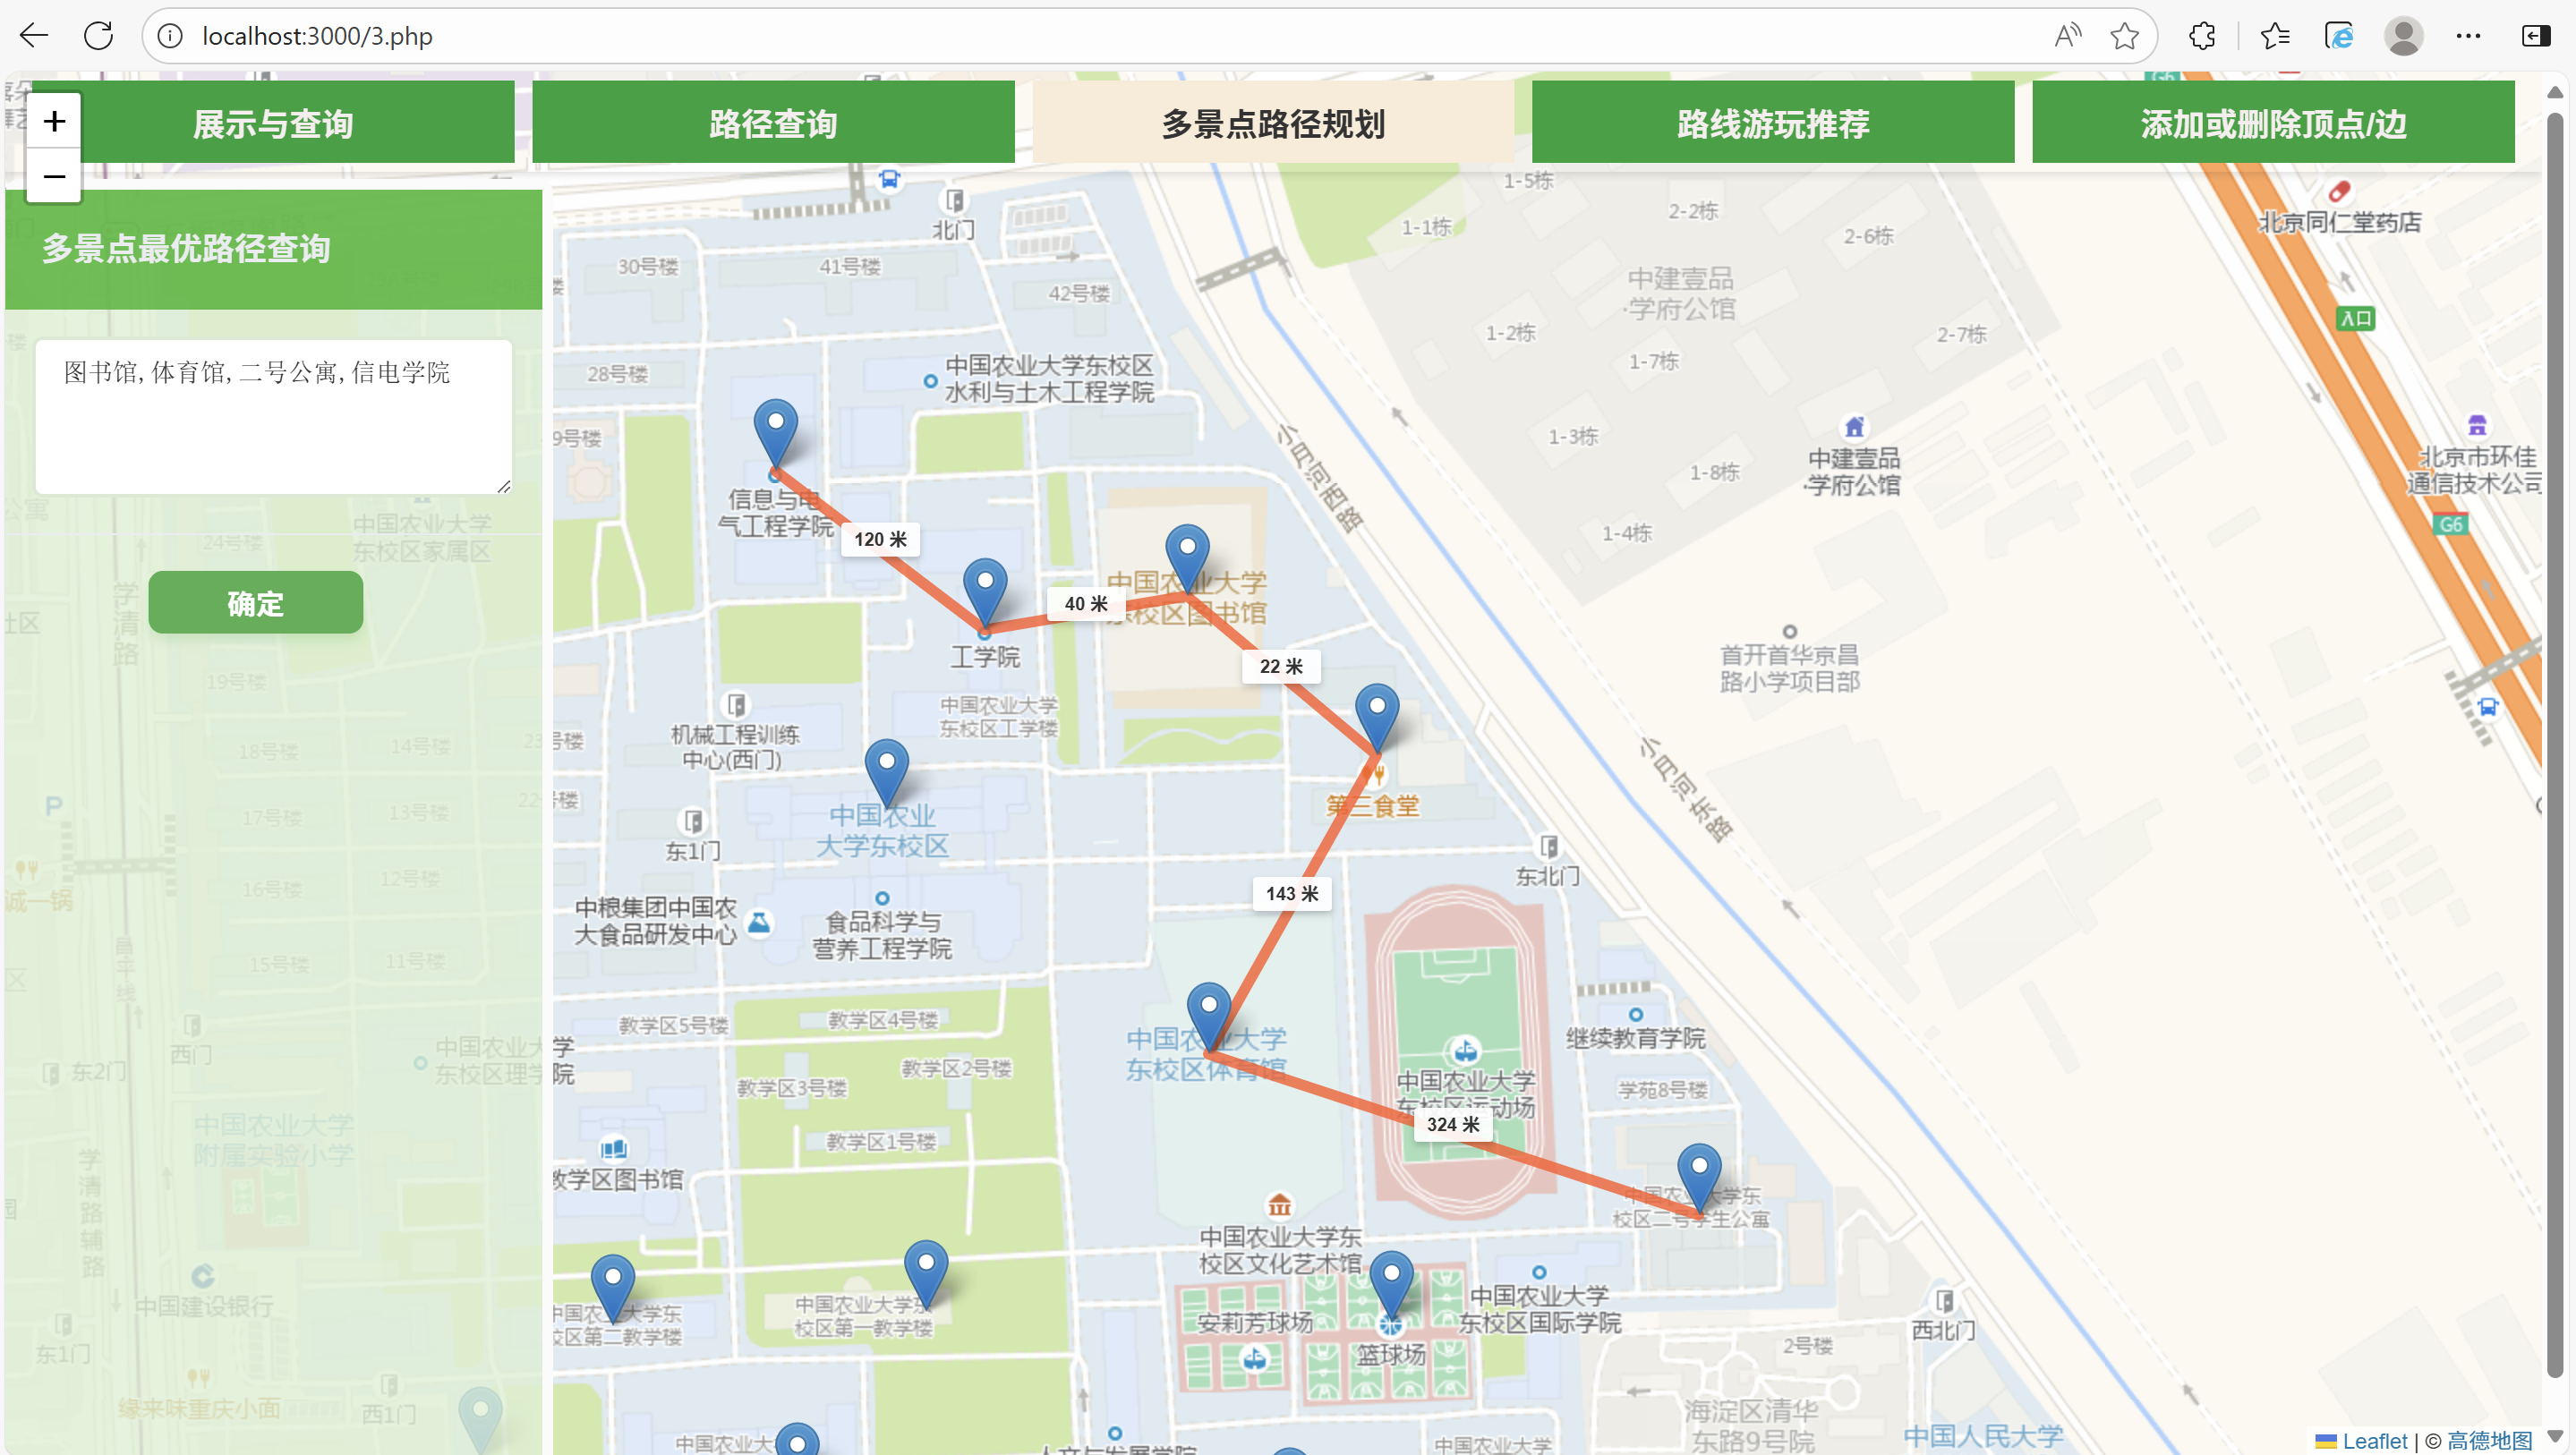
\includegraphics[width=0.9\textwidth]{figures/3.png}
\caption{多景点路径规划展示}\label{fig:f5}
\end{figure}

\subsubsection{多景点路径规划的算法内容与算法分析}

算法的核心思想是采用\textbf{压缩策略}，在n-Floyd表的
基础上进行压缩，将未出现在要求\textbf{必经景点(k)}中的点剔除在边界
之外，由于我们需要完整路径，所有我们将顶点挂在
裁剪后的k-Floyd表的后面，做成悬挂边式的Floyd表。
这是我们专门为此设计的新的数据结构。

具体数据结构形式如下：

\begin{tcode}
    typedef struct floyd{
        // length 指的是每条边的长度
        int num;
        floyd* next;
        floyd() : num(0), next(nullptr) {}
        floyd(int n) : num(n), next(nullptr) {}
        void push_back(int k) {
            floyd* p = this;
            while (p->next != NULL) p = p->next;
            p->next = new floyd;
            p->next->num = k;
        }
    }floyd;

    class contra_Floyd_hanging {
    private:
        floyd** form;
        // 第一个 num 指的是每条边的长度，后面的 num 是悬挂点的序号
    public:
    ……
    };
\end{tcode}

在这个数据结构的基础上，我们进行算法设计。
我们采用压缩的方法，将n-Floyd压缩成k-Floyd带边表。
核心在于压缩过程，实际上是通过读paths矩阵，来获取路径。

\begin{tcolorbox}[mydashedbox]
WHILE(TRUE)

a.取任意两个k中点，如果读出的路径中没有k中其他点，
那就将所有点全部拉到悬挂边上。然后退出while循环。

b.如果存在其他k中点，断开，根据最短路径中任意两点间仍最短的子问题结构，
将前半部分直接悬挂在i-k对应位置，将k-j段重新执行上述选择。
\end{tcolorbox}

利用get，fg，fg\_form三个类指针进行扫描，
get指针用于标定现在的起始点，fg指针用于标定向前伸展地抵达的点，
fg\_form用于标定前一个点，从而和fg比对确认是否抵达终点。

\subsubsection{TSP算法求解悬挂边表矩阵}

然后对悬挂边表进行TSP算法处理。首先，由于k为
必须至少经过的点，一般来说实际应用中较少，
所有我尝试使用暴力法直接求解TSP，
输出全排列直接求结果，
实际复杂度$O(n!)$。
根据实测，在第11个点是需要分钟级别时间，第12个点时
会占用大量电脑的CPU资源无法短时间跑出。

所以队友写了一个dp-TSP算法，
我将其套用在悬挂边表的数据结构上，
顺利实现了极短时间内跑完我们所有的13个点。
时间复杂度理论上$O(n^2 \cdot 2^n)$，
由于dp-TSP为队友所写，我就不过多赘述了。

\subsubsection{多景点路径规划算法时间复杂度分析}

此算法分为三部分，\textbf{n-Floyd矩阵的求解
、k-Floyd矩阵压缩算法、k-TSP求解算法}。
n-Floyd矩阵的求解时间复杂度为$O(n^3)$（具体原因已讲解）；

k-Floyd矩阵压缩算法的时间复杂度首先由于要遍历k*k维矩阵，
在每个分类求解时存在一个while循环，循环数最多不超过所有顶点n。
所以时间复杂度为$O(k^2\cdot n)$；

当k-TSP以dp算法求解时，时间复杂度为$O(k^2\cdot 2^k)$。

总时间复杂度为$O(n^3+k^2\cdot n+k^2\cdot 2^k)$，
而和上面2.1部分一样，n-Floyd矩阵仅每次增删改变
新点时进行改变，其他时候直接调用，
不涉及改变时直接执行此算法时间复杂度为
$O(n\cdot k^2+k^2\cdot 2^k)$，k一般一定不会很大，
所以这个时间复杂度实际上很小！

\subsection{路线游玩推荐页面}

对路线游玩推荐功能，
我们考虑创新式的引入
旅游者最大时间的限制和最大化效益的
目标。对于最大时间限制有两种考虑，
构成了下面的两种初始模型。

一种是单纯考虑时间是一个临界因子，
假设它是一个硬性约束。将约束转化为优化问题。
从而考虑最小化时间，最大化旅游效益。

另一种是考虑时间一定是一个先增后减的凸函数（由于反馈
机制和心理学研究进行的合理猜测）。
通过多目标因子优化和寻找在最大时间限制下最优的游玩时间
长度。


\subsubsection{多目标规划模型-模型1}
对于路线游玩\textbf{推荐}，我们首先
考虑对于这种推荐的观光者问题，
我们首先分析推荐的目标，
以\textbf{时间花费总数不超过限制时间}为约束，
将约束转化为优化问题。从而考虑最小化时间
\textbf{最大化个人享受的效益}。
对于这样的要求，建立公式化模型如下：

\begin{equation}
    \begin{aligned}
        & max\quad w_1 \cdot n_{revenue} +
        w_2 \cdot \frac{1}{Time} \\
        & s.t. \begin{cases}
            n_{revenue} = \sum_{i=0}^{n} n_i \\
            Time = \sum_{i=0}^{n} visitTime
             + \sum_{i=0}^{n-1} \frac{lens[i][i+1]}{vector} \\
            Time \leq T_{max} \\
            w = [w_1, w_2]\quad \text{为权重两目标权重向量} \\
            visitTime = [...]\quad \text{每类人景点停留时间} \\
            lens = [...][...]\quad \text{景点间步行距离} \\
            vector\quad \text{每类人步行速度},~T_{max}\quad \text{最大时间}
        \end{cases}
    \end{aligned}
\end{equation}

\subsubsection{多目标规划模型-模型2}

我们首先考虑一个先增后减的函数，
$y=\frac{x}{e^x}$符合这个趋势，进行变换，
得到函数$y=\frac{At}{e^{\theta t}}$。
很容易推导出，实际上不同人群对时间利用率的忍耐程度有差别，
通过给定不同人群参数k（最大能接受为最高时间效益的比例），
可以推导出公式：

\begin{figure}[!h]
\centering
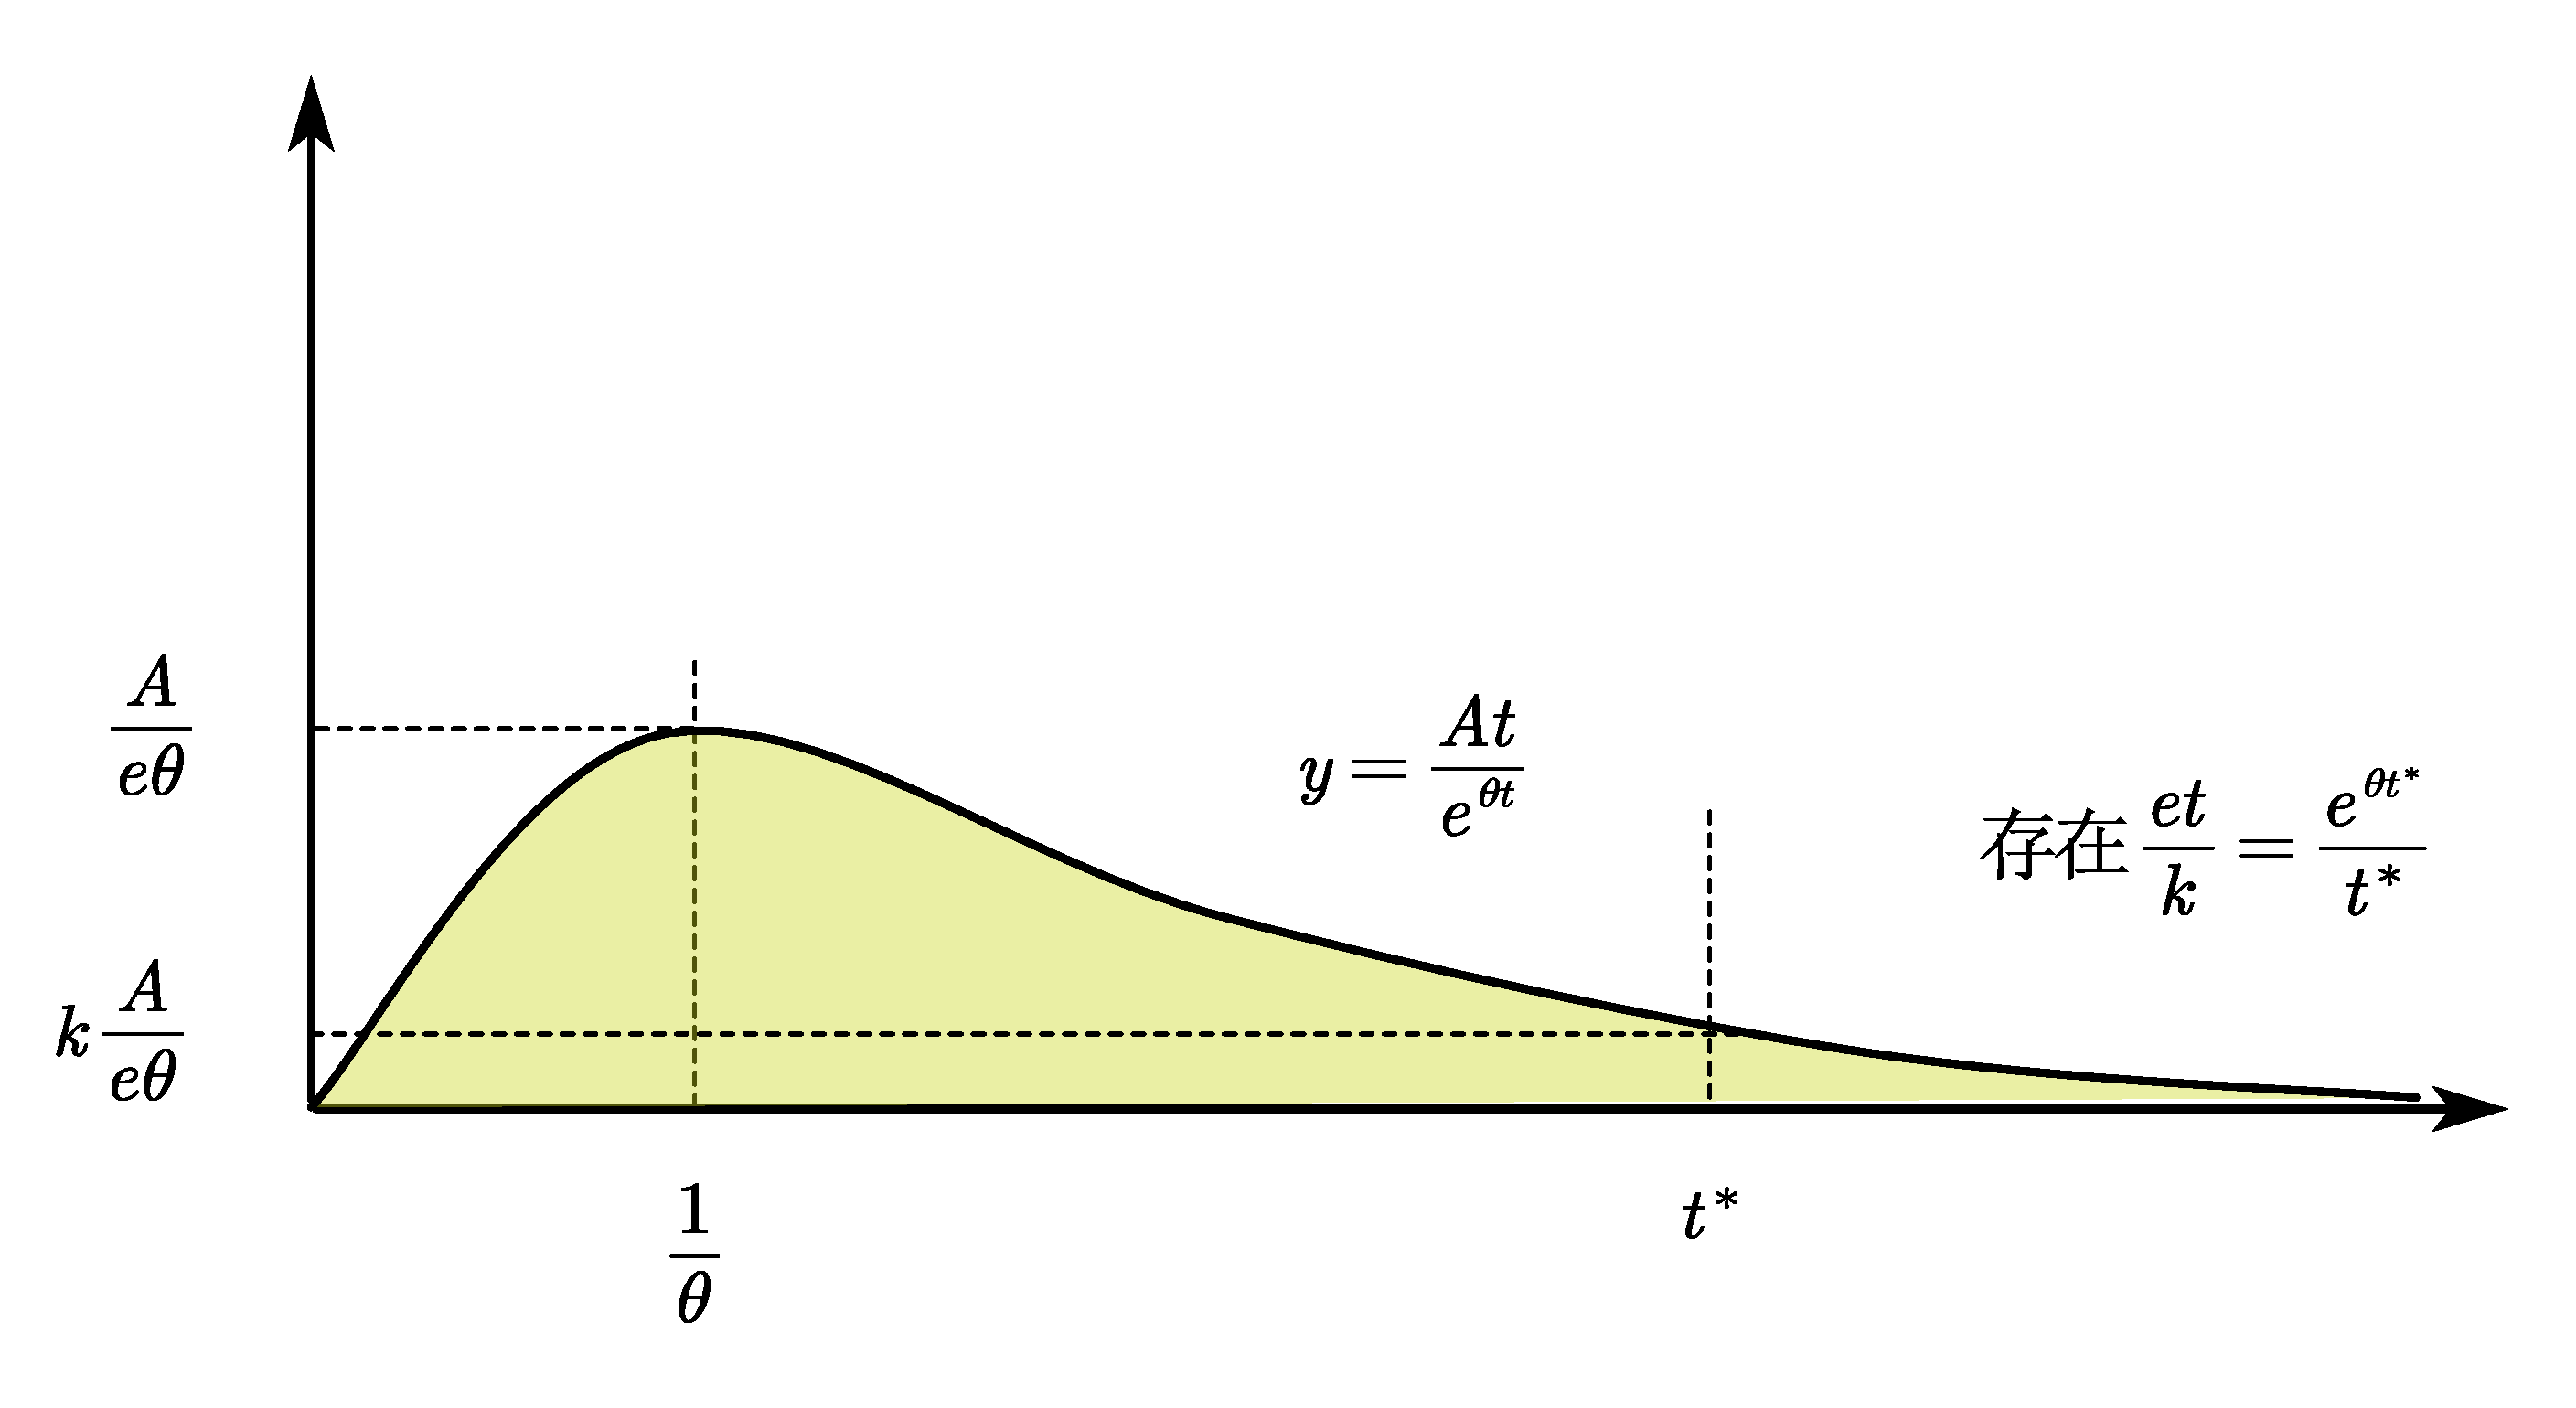
\includegraphics[width=0.9\textwidth]{figures/model2.pdf}
\caption{时间变化机理图展示}\label{fig:f6}
\end{figure}


\begin{equation}
    \begin{aligned}
        & min\quad w_1\cdot \frac{1}{n_{revenue}} + w_2 \cdot d^{-} + w_3 \cdot d^{+} \\
        & \begin{cases}
            n_{revenue} = \sum_{i=0}^{n} n_i \\
            Time = \sum_{i=0}^{n} visitTime
             + \sum_{i=0}^{n-1} \frac{lens[i][i+1]}{vector} \\
            \frac{et}{k}=\frac{e^{\theta t^*}}{t^*} \\
            Time + d^{-} + d^{+} = t^* \\
            \text{其他参量定义与模型1一致}
        \end{cases}
    \end{aligned}
\end{equation}

主要区别点在猜测了一个时间效益下降函数，
将最大时间约束转化为最优时间约束
以及将尽可能小改为尽可能接近。


\subsubsection{蚁群算法模型}
针对上面的多目标规划推荐问题，
如果采取穷举方法的时间复杂度求解如下：

由于可以是任意景点的任意组合，
所以排列种类为为$\sum_{i=0}^{n} A_n^i\approx 
e\cdot A_n^n \approx 2.7\cdot n!$，
时间复杂度为$O(2.7 \cdot n!)$。

是一个较高复杂度下的算法，
根据上面的经验$n \geq 12$是已经无法暴力求解，
这里采用群智能算法中的蚁群算法来进行求解。

蚁群算法的基本原理如下：

\begin{equation}
    \begin{cases}
        \textbf{信息素变化} \\
        \eta_{ij} = \frac{n_j}{\frac{lens_{ij}}{vector} + visitTime_j + \varepsilon} \\
        \tau_{ij}(t+1) = (1 - \rho) \cdot \tau_{ij}(t) \\
        \tau_{ij}(t+1) = \tau_{ij}(t+1) + \sum_{k=1}^{m} \Delta\tau_{ij}^k \\
        \textbf{从i到j的变化量} \\
        \Delta\tau_{ij}^k = 
            \begin{cases}
            \dfrac{Q \cdot n_{revenue}[k]}{\text{sum\_enjoy\_upper}}, & \text{如果蚂蚁}k\text{经过边}(i,j)\\
            0, & \text{else}
            \end{cases} \\
        \textbf{状态转移概率} \\
        p_{ij}^k = 
            \begin{cases}
            \dfrac{[\tau_{ij}(t)]^\alpha \cdot [\eta_{ij}]^\beta}{\sum\limits_{l \in \mathcal{N}_i^k} [\tau_{il}(t)]^\alpha \cdot [\eta_{il}]^\beta}, & \text{如果蚂蚁可行j}\\
            0, & \text{else}
            \end{cases}
    \end{cases}
\end{equation}

\subsubsection{蚁群算法的复杂度分析}
对于蚁群算法，每只蚂蚁构建路径的时间为$O(n^2)$，
共m只蚂蚁，故为$O(m\cdot n^2)$，
由于迭代k此，故总的时间复杂度为
$O(k\cdot m \cdot n^2)$。

\subsubsection{推荐游玩页面展示}

\begin{figure}[!h]
\centering
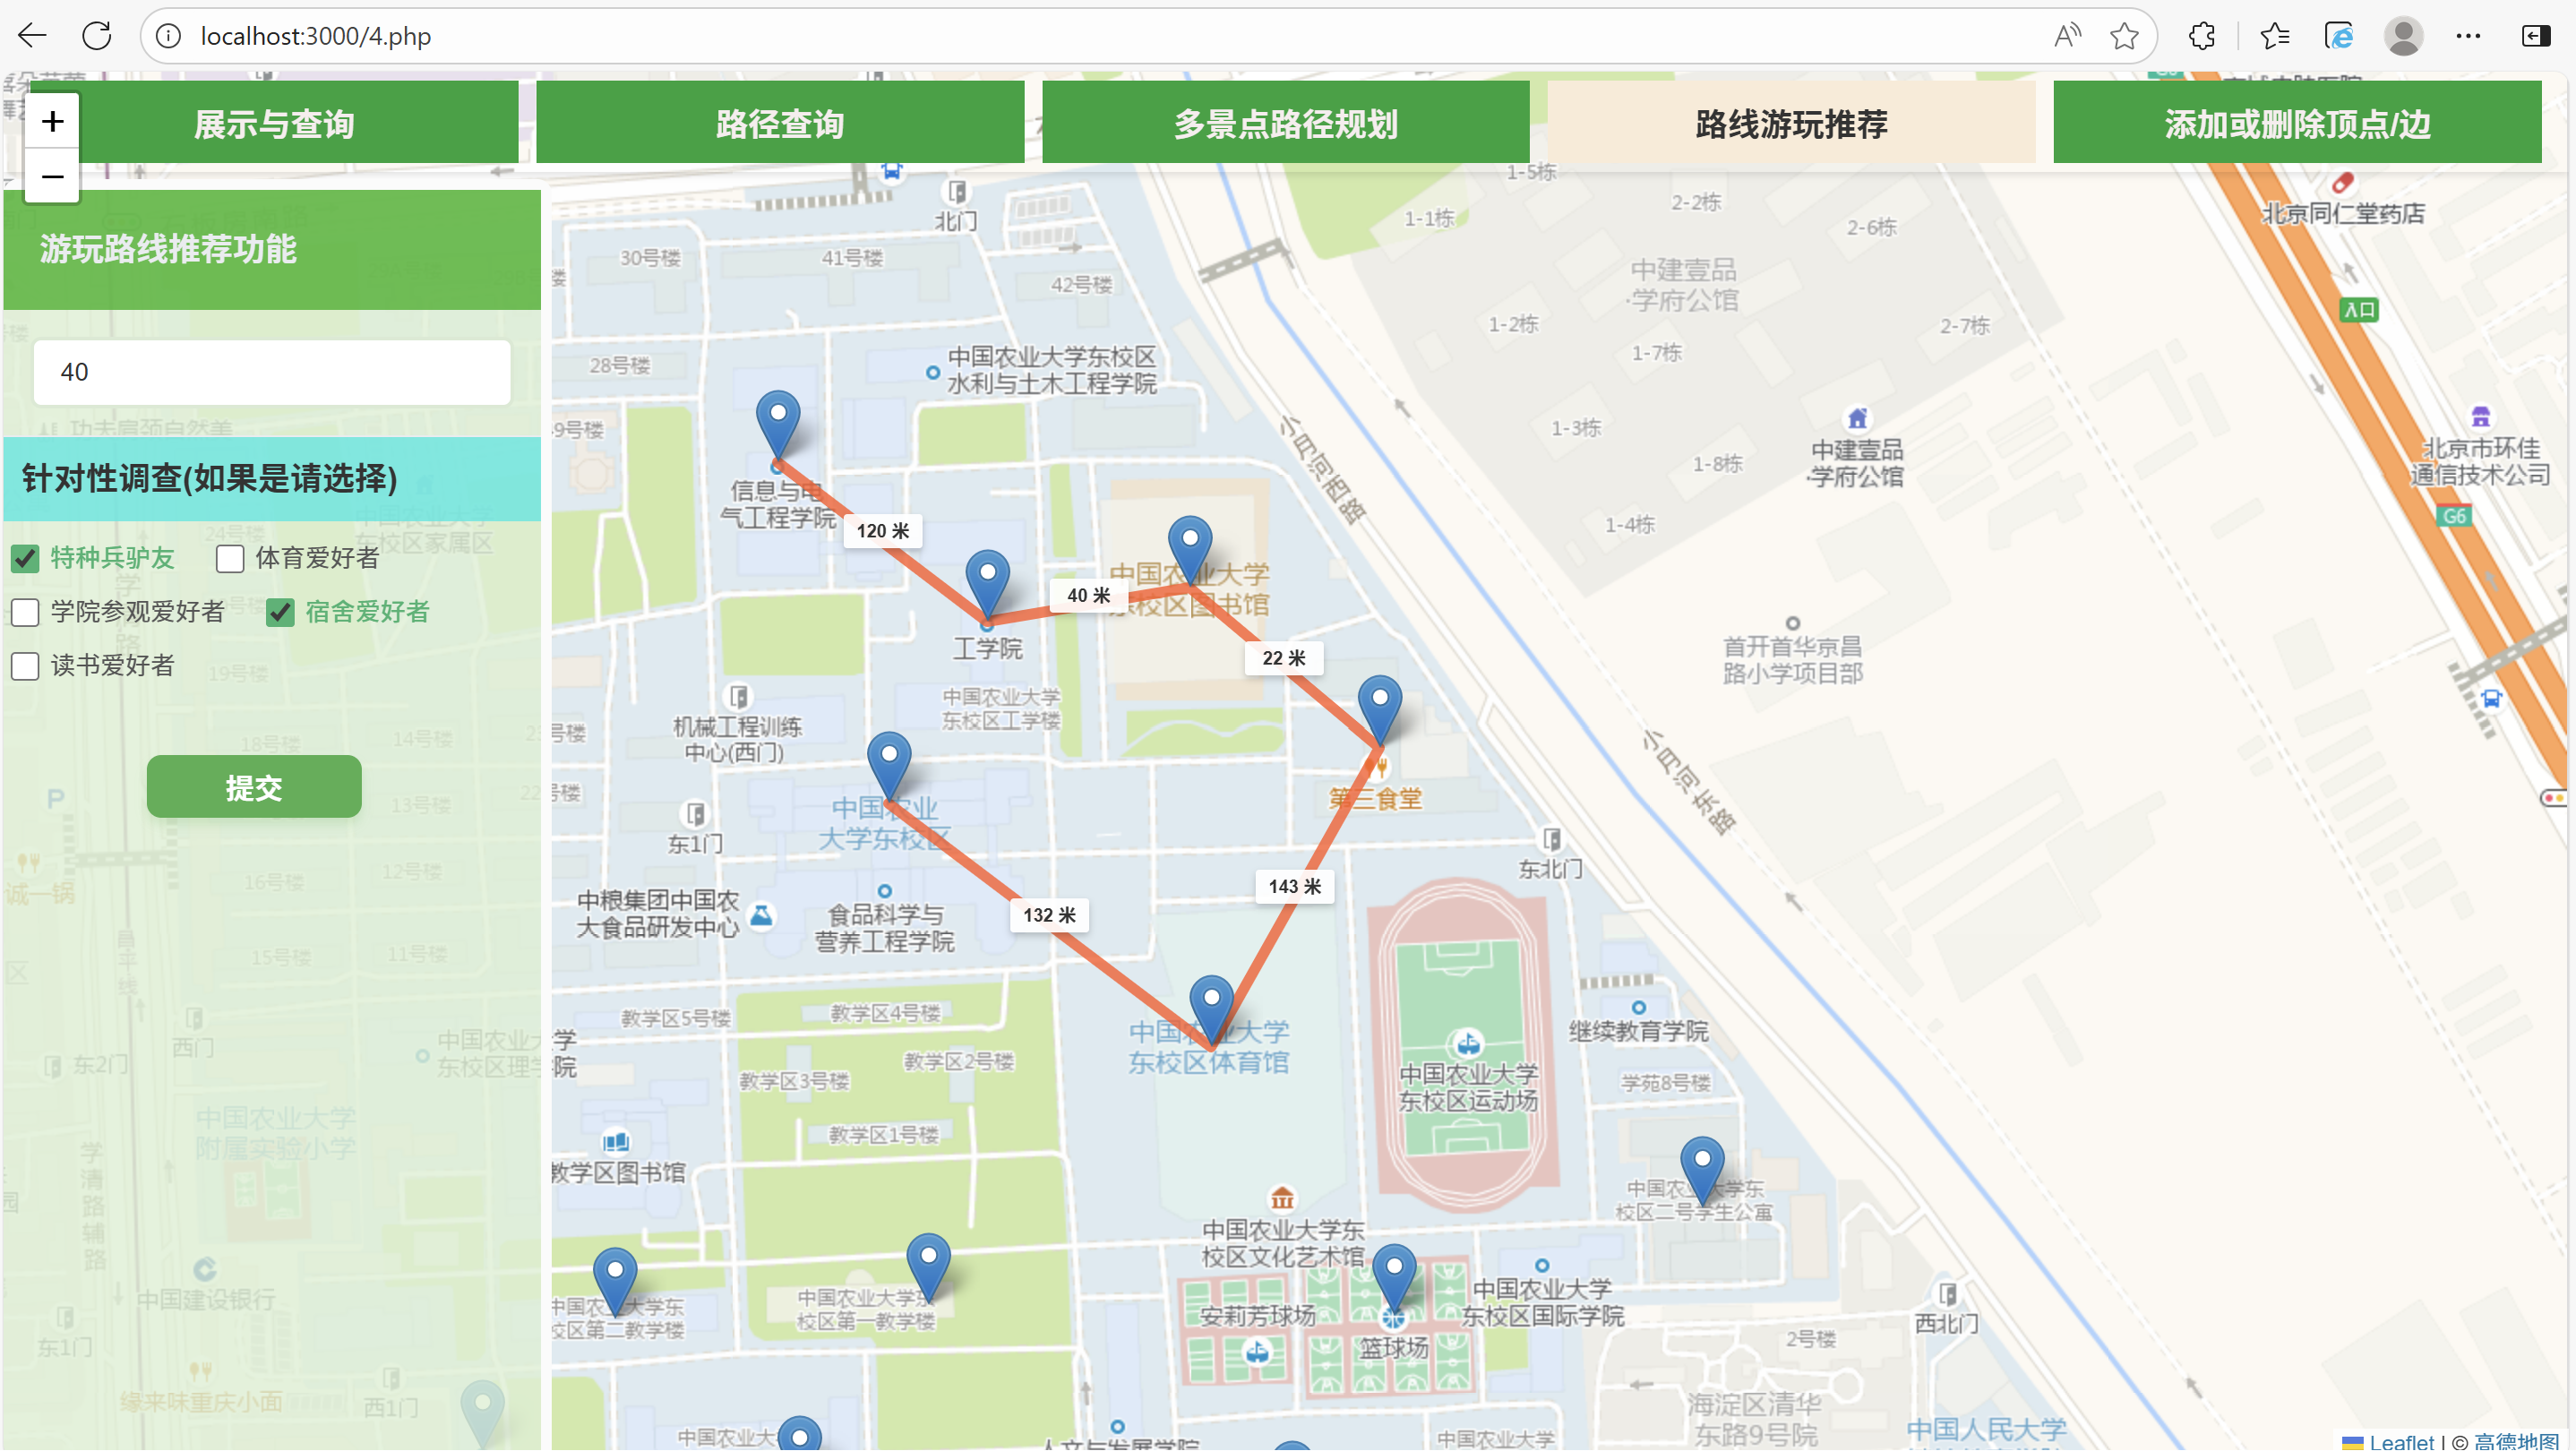
\includegraphics[width=0.9\textwidth]{figures/4-1.png}
\caption{推荐页面展示1}\label{fig:f6}
\end{figure}

\begin{figure}[!h]
\centering
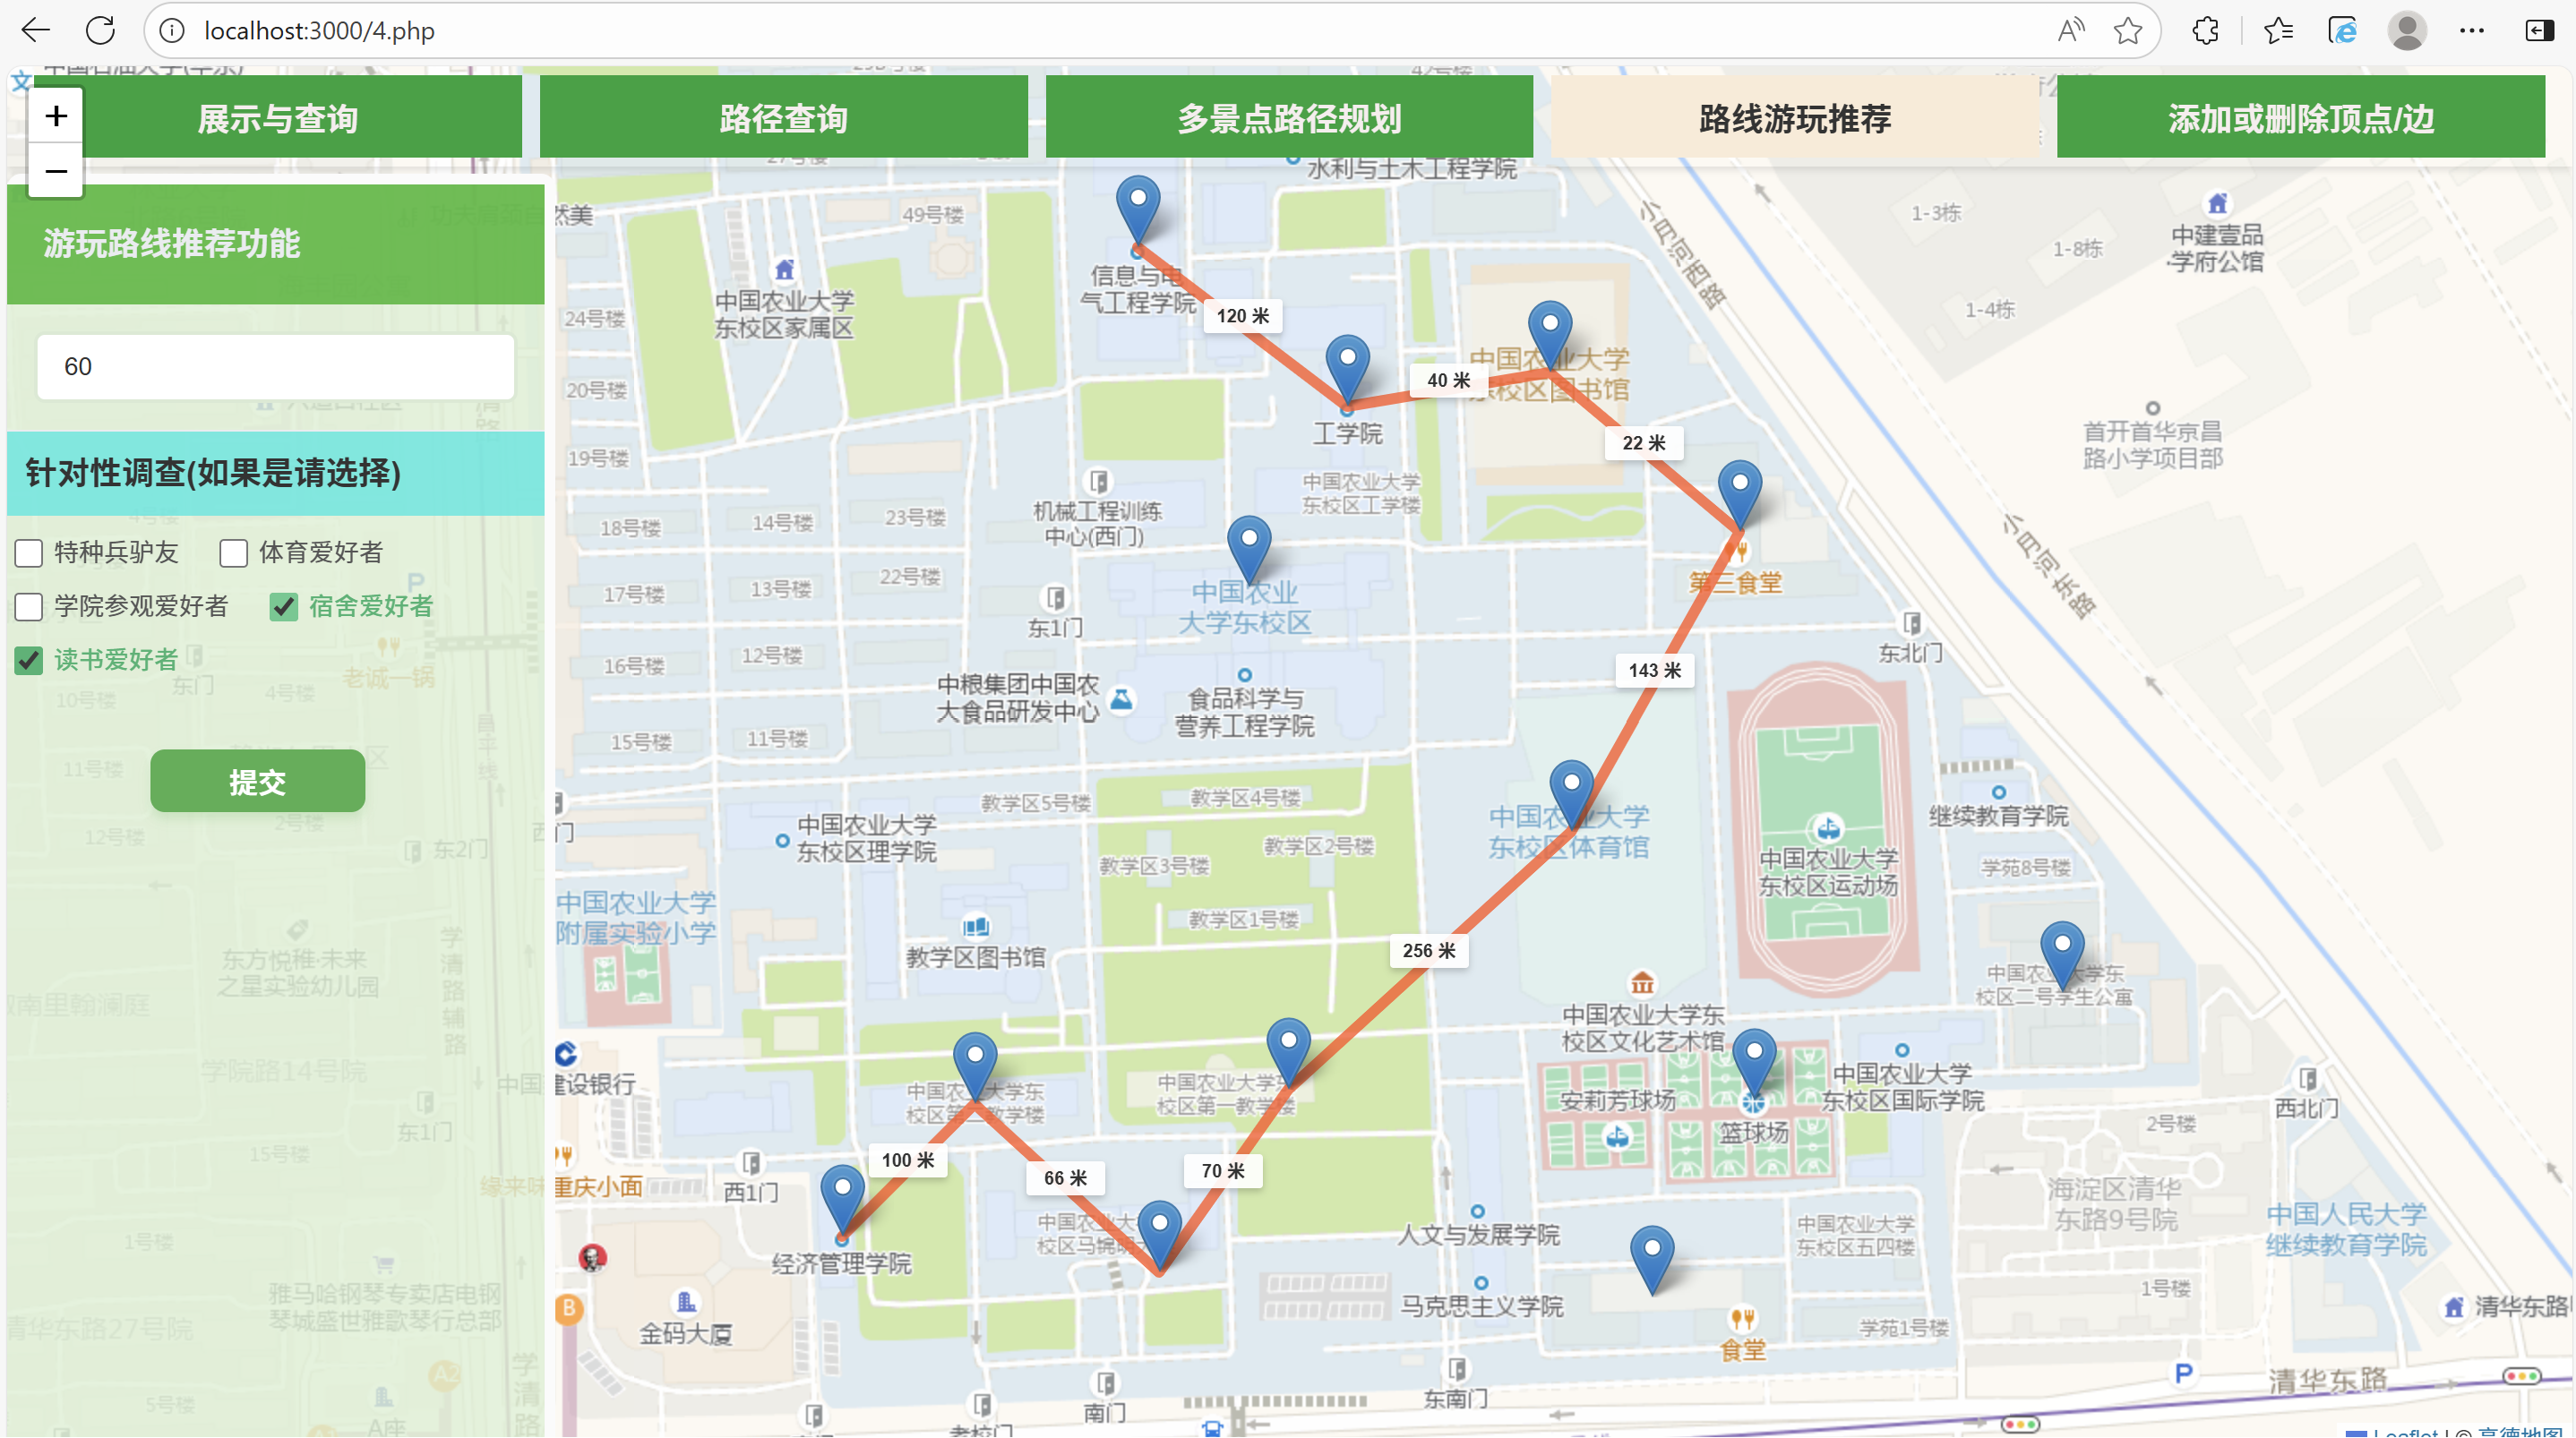
\includegraphics[width=0.9\textwidth]{figures/4-2.png}
\caption{推荐页面展示2}\label{fig:f7}
\end{figure}

\newpage

\section{算法设计分析}
由于在第二部分已经完整的梳理了整个算法流程，
各个部分的分析已经比较完整，
下面我们简要归纳一下各部分内容。


\subsection{原始模型}
对于原始算法模型，
即直接采用现有的算法模型带入到我们工程
的模型。我负责的部分是包括：

\textbf{算法方面的}Floyd算法，暴力TSP，
群智能蚁群算法。这些算法保留传统模型没有做
太多的优化。主要是在我们的系统中应用。

\textbf{工程方面的}C++与php的
数据交互函数，由于二者不像python和php可以通过json互换，
只能将二者均转化为字符串形式进行转换，各自再分别拆解识别。
以及php和javascript的数据交互，还有页面的主要代码书写。
包括leaflet的调用，路线的可视化展示和html呈现。

\subsection{扩展优化模型}
而对于扩展模型，在基本的算法基础上作修正改进，
我主要负责的有：

多景点路径规划开发了一套对已有的n-Floyd表进行
压缩的算法，时间复杂度较好。同时恰当的
实现了“长”出一条最短路径的任务。

多目标规划算法，提出了两个可使用
模型，一个是转化成两个最大化问题，
一个是转化为极小紧邻区间约束问题。
可以很好的解决问题。


\subsection{特殊处理}
值得一提的特殊处理是建立了k-Floyd带边表的数据结构。
建立起这样一个C++类，
便捷的实现了上述的多景点路径规划任务。

除此以外，多目标规划中对于时间效益
根据现实形式和心理学考虑，猜测了一个先升再降的凸函数，
从而希望更好的描述时间约束，
处理比较特殊。


\subsection{算法复杂度分析}

\begin{table}[!htbp]
    \caption{算法复杂度分析表格}\label{tab:tab1}
    \centering
    \begin{tabular}{lcccc}
        \toprule[1.5pt]
        \textbf{算法名称} & \textbf{Floyd算法} & \textbf{暴力TSP} & \textbf{压缩算法} & \textbf{蚁群算法} \\
        \midrule[1pt]
        \textbf{时间复杂度} & $O(n^3)$ & $O(n!)$ & $O(n \cdot k^2)$ & $O(k\cdot m \cdot n^2)$ \\
        \textbf{空间复杂度} & $O(n^2)$ & $O(n)$ & $O(n\cdot k^2)$ & $O(n^2 + m\cdot n)$ \\
        \bottomrule[1.5pt]
    \end{tabular}
\end{table}




\section{调试分析}
\subsection{关键代码段说明}

除了在二中梳理时展示的Floyd核心算法，k-Floyd带边表数据结构代码段，
其他的算法核心代码由于较长所以放在附录B中。工程核心代码在附件中。

\subsection{调试过程}

调试过程演示，主要是在网页，vs，exe间的协调。

\begin{figure}[!h]
\centering
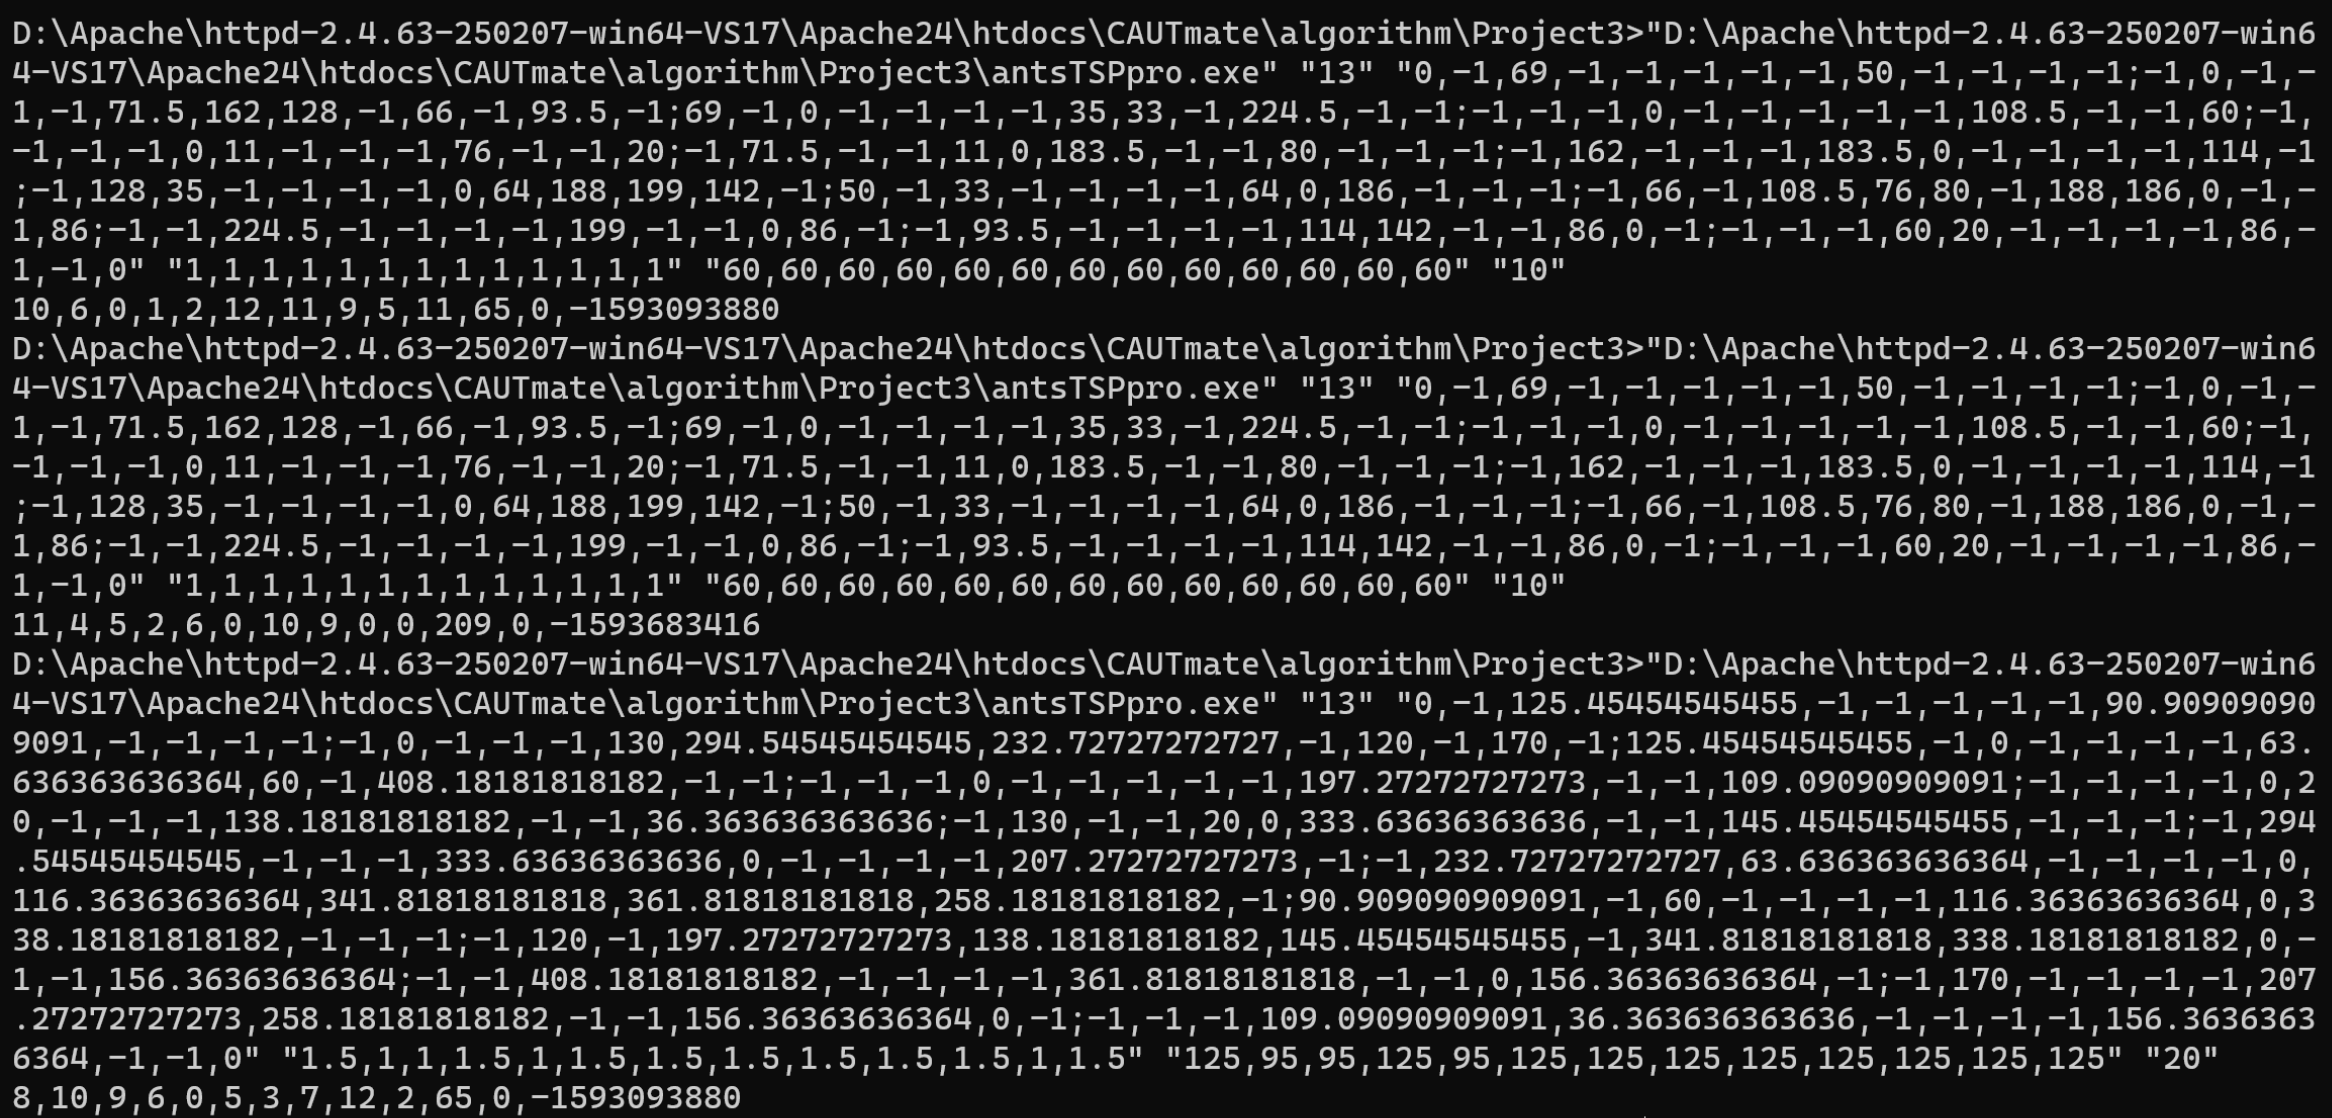
\includegraphics[width=0.9\textwidth]{figures/image00.png}
\caption{调试页面展示}\label{fig:f8}
\end{figure}




\section{未来发展方向和想法}

在大数据下我们可以做错峰分配、路径调度，在现实应用程序中我们可以做
时间、地点、用户画像下的合理多条推荐与跳转（比如高德的团购推荐就是导游软件的服务生态
打造）。未来在农大导览和推荐方面，主要是围绕农大特色与情景需要（由于作为景点农大客流量较少），
我们可以考虑新生入学的导览系统，历史的相关介绍与推荐，以及集成导游相关信息，
创造圈层生态的一个方向。

在呈现形式上，可以与信息提供的社交平台组合，整合信息与导览生态。
瞄定高目标的路径规划、信息获取、社交绑定需求。







\section*{参考文献}

\renewcommand{\refname}{} % 清空参考文献标题
\begin{thebibliography}{9}

\bibitem{c1}
毛晨希, 高成栋, 宋瑾钰. 基于蚁群算法的多约束动态旅游路线规划[J]. 运筹与模糊学, 2023, 13(2): 1082-1093. 
\\https://doi.org/10.12677/ORF.2023.132112s
\bibitem{c2}
王文成，王曦雅，牛秦州，等. 基于逻辑模型的多偏好旅游路线规划研究[J]. 现代电子技术，2025，48（7）：169⁃176.

\end{thebibliography}



\newpage
%附录
\begin{appendices}

\section{工程结构说明}

\begin{mdframed} [%
	roundcorner=5pt,
	linecolor=gray!50,
	outerlinewidth=0.5pt,
	middlelinewidth=0.3pt, backgroundcolor=gray!2,
innertopmargin=\topskip, frametitle={工程结构说明},
frametitlefont= \bfseries,frametitlerule=true,frametitlealignment =\raggedright\noindent,
frametitlerulewidth=.5pt, frametitlebackgroundcolor=gray!2,]
具体汇总工程结构如下
\begin{enumerate}
\item css \begin{enumerate}
        \item 1.css （同时作为index.php和1.php的css文件）
        \item 2.css
        \item 3.css
        \item 4.css 
    \end{enumerate}
\item index.php 主页面，用于展示各点信息和实际图点位
\item 1.php （index.php的变体，用于展示所有路径）
\item 2.php 用于实现两点间1条或多条或所有路径查询
\item 3.php 用于实现至少经过某些顶点的最短路径查询
\item 4.php 用于实现推荐不同人群在最大限时下的最优路径
\item Floyd.exe
\item yens.exe
\item DFS.exe
\item polyscenespro.exe
\item antsTSPpro.exe
\item C++源文件
\end{enumerate}
\end{mdframed}


\section{算法部分代码}

\noindent 注：工程代码请见支撑材料

\subsubsection{多景点路径规划算法}

\begin{tcode}

typedef struct floyd{
	// length 指的是每条边的长度
	int num;
	floyd* next;
	floyd() : num(0), next(nullptr) {}
	floyd(int n) : num(n), next(nullptr) {}
	void push_back(int k) {
		floyd* p = this;
		while (p->next != NULL) p = p->next;
		p->next = new floyd;
		p->next->num = k;
	}
}floyd;

class contra_Floyd_hanging {
private:
	floyd** form;
	// 第一个 num 指的是每条边的长度，后面的 num 是悬挂点的序号
public:
	contra_Floyd_hanging(int n) {
		form = new floyd * [n];
		for (int i = 0; i < n; i++) {
			form[i] = new floyd[n];
		}
		for (int i = 0; i < n; i++) {
			for (int j = 0; j < n; j++) {
				form[i][j].num = 0;
			}
		}
	}
	int get_length(int x, int y) {
		return form[x][y].num;
	}
	void change_length(int x, int y, int k) {
		form[x][y].num = k;
	}
	floyd* rear(int x, int y) {
		floyd* p = &form[x][y];
		while (p->next != NULL) p = p->next;
		return p;
	}
	void push_back(int x, int y, int k) {
		floyd* p = &form[x][y];
		while (p->next != NULL) p = p->next;
		p->next = new floyd;
		p->next->num = k;
	}
	void push(int x, int y, floyd* k) {
		form[x][y].next = k->next;
	}
	floyd* next(int x, int y) {
		return form[x][y].next;
	}
};

int index(int* a, int n, int x) {
	bool status = false;
	int i = 0;
	for (i = 0; i < n; i++) {
		if (a[i] == x) {
			status = true;
			break;
		}
	}
	return i;
}

bool in(int* a, int n, int x) {
	bool status = false;
	for (int i = 0; i < n; i++) {
		if (a[i] == x) {
			status = true;
			break;
		}
	}
	return status;
}


// 采用边界收缩策略，路径重排，剥离(隐藏/悬挂)不需要的点--在最后的最简连接表上悬挂隐藏点
void poly_scenes_pro(int** Floyd_length, int** Floyd_path, int* points, int num, contra_Floyd_hanging &form) {
	// 压缩为 Floyd 悬挂表

	for (int i = 0; i < num; i++) {
		for (int j = 0; j < num; j++) {
			int i_true = points[i];
			int j_true = points[j];

			if (i == j) continue;
			else {
				if (form.get_length(i, j) != 0) continue;
				else {
					int get = i_true;
					int fg_form = i_true;
					floyd* pin_edge = new floyd(0);
					int fg;

					while (true) {
						// 发现对Floyd算法理解错误
						// 3->9->8->0 输3->0首先得到靠近3的9
						fg = Floyd_path[fg_form][j_true];
						if (fg_form == get) {
							if (fg_form == fg) {
								form.change_length(index(points, num, get), j, Floyd_length[get][j_true]);
								form.push(index(points, num, get), j, pin_edge);
								break;
								// 这个时候悬挂一定为空
							}
							else {
								if (in(points, num, fg)) {
									form.change_length(index(points, num, fg_form), index(points, num, fg), Floyd_length[fg_form][fg]);
									form.push(index(points, num, fg_form), index(points, num, fg), pin_edge);
									fg_form = fg;
									get = fg;
									// 这个时候悬挂一定为空
								}
								else {
									fg_form = fg;
									pin_edge->push_back(fg);
								}
							}
						}
						else {
							if (fg_form == fg) {
								// 这里的fg_form不可能in points, 因为如果in的话先前就回导向回ff = fg = get
								// push_back(fg) 这个地方不应该再追加!!!!
								form.change_length(index(points, num, get), j, Floyd_length[get][j_true]);
								form.push(index(points, num, get), j, pin_edge);
								break;
							}
							else {
								if (in(points, num, fg)) {
									form.change_length(index(points, num, get), index(points, num, fg), Floyd_length[get][fg]);
									form.push(index(points, num, get), index(points, num, fg), pin_edge);

									pin_edge = new floyd(0);
									fg_form = fg;
									get = fg;
								}
								else {
									pin_edge->push_back(fg);
									fg_form = fg;
								}
							}
						}
					}
				}
			}
		}
	}
\end{tcode}

\subsubsection{多目标规划蚁群算法}

\begin{tcode}
struct Ant {
    vector<int> path;
    vector<bool> visited;
    double time_total = 0.0;
    double enjoy_total = 0.0;
    double utility = -1e100;
};


string ant_multi_points_tsp(int N, double** dist, double* enjoy,
    double* visit_time, double T_max) {
    // 处理 dist 矩阵的 -1
    for (int i = 0; i < N; i++) {
        for (int j = 0; j < N; j++) {
            if (dist[i][j] == -1) dist[i][j] = INF;
        }
    }


    string result = "";

    // ---- ACO 参数 ----
    int ITER = 400;
    int ANTS = max(20, N);
    double alpha = 1.0;
    double beta = 3.0;
    double rho = 0.25;
    double Q = 10;
    double w = 0.5;
    unsigned seed = (unsigned)chrono::high_resolution_clock::now().time_since_epoch().count();
    mt19937 rng(seed);
    uniform_real_distribution<double> urand(0.0, 1.0);


    vector<vector<double>> tau(N, vector<double>(N, 1.0));
    // 转移效益--启发式函数
    auto heuristic = [&](int i, int j)->double {
        double denom = dist[i][j] + visit_time[j] + 1e-9;
        return (enjoy[j] <= 0.0 ? 1e-9 : enjoy[j]) / denom;
        };

    double sum_enjoy_upper = 0.0;
    for (int i = 0; i < N; i++) sum_enjoy_upper += max(0.0, enjoy[i]);
    if (sum_enjoy_upper <= 0) sum_enjoy_upper = 1.0;

    vector<int> best_path_global;
    double best_utility_global = -1e100;
    double best_time_global = 0.0, best_enjoy_global = 0.0;

    // ---- 蚂蚁构造函数 ----
    auto construct_ant = [&](Ant& ant) {
        ant.path.clear();
        ant.visited.assign(N, false);
        ant.time_total = 0.0;
        ant.enjoy_total = 0.0;
        ant.utility = -1e100;

        int cur = rng() % N;
        ant.path.push_back(cur);
        ant.visited[cur] = true;
        ant.time_total += visit_time[cur];
        ant.enjoy_total += max(0.0, enjoy[cur]);

        while (true) {
            vector<int> cand;
            vector<double> score;
            double sum_score = 0.0;

            for (int j = 0; j < N; ++j) {
                if (ant.visited[j]) continue;
                double extra_time = dist[cur][j] + visit_time[j];
                if (ant.time_total + extra_time <= T_max) {
                    double s = pow(tau[cur][j], alpha) * pow(heuristic(cur, j), beta);
                    if (s < 1e-18) s = 1e-18;
                    cand.push_back(j);
                    score.push_back(s);
                    sum_score += s;
                }
            }

            if (cand.empty()) break;

            double r = urand(rng) * sum_score;
            int sel = 0;
            for (int idx = 0; idx < (int)cand.size(); ++idx) {
                r -= score[idx];
                if (r <= 0) { sel = idx; break; }
                if (idx == (int)cand.size() - 1) sel = idx;
            }
            int nxt = cand[sel];

            ant.path.push_back(nxt);
            ant.visited[nxt] = true;
            ant.time_total += dist[cur][nxt] + visit_time[nxt];
            ant.enjoy_total += max(0.0, enjoy[nxt]);
            cur = nxt;
        }

        if (ant.time_total > T_max + 1e-9) {
            ant.utility = -1e100;
        }
        else {
            double norm_enjoy = ant.enjoy_total / sum_enjoy_upper;
            double norm_time = ant.time_total / max(1e-9, T_max);
            ant.utility = w * norm_enjoy - (1.0 - w) * norm_time;
        }
        };

    auto deposit_pheromone = [&](const vector<int>& path, double amount) {
        if (amount <= 0) return;
        for (size_t i = 0; i + 1 < path.size(); ++i) {
            int u = path[i], v = path[i + 1];
            tau[u][v] += amount;
            // 如果图是无向的，可以加上：
            // tau[v][u] += amount;
        }
        };

    // 主循环
    for (int it = 0; it < ITER; ++it) {
        vector<Ant> ants(ANTS);
        for (int k = 0; k < ANTS; ++k) {
            construct_ant(ants[k]);
        }

        for (int i = 0; i < N; ++i)
            for (int j = 0; j < N; ++j)
                tau[i][j] *= (1.0 - rho);

        Ant best_iter_ant;
        best_iter_ant.utility = -1e100;

        for (int k = 0; k < ANTS; ++k) {
            if (ants[k].utility <= -1e90) continue;
            double base = Q * (ants[k].enjoy_total / (sum_enjoy_upper + 1e-9));
            deposit_pheromone(ants[k].path, base);

            if (ants[k].utility > best_iter_ant.utility) best_iter_ant = ants[k];
            // 这里储存了最优解---蚁群算法有最优记忆性!!!!
        }

        if (best_iter_ant.utility > -1e90) {
            deposit_pheromone(best_iter_ant.path, Q * 2.0);
        }

        if (best_iter_ant.utility > best_utility_global) {
            best_utility_global = best_iter_ant.utility;
            best_path_global = best_iter_ant.path;
            best_time_global = best_iter_ant.time_total;
            best_enjoy_global = best_iter_ant.enjoy_total;
        }

        for (int i = 0; i < N; ++i)
            for (int j = 0; j < N; ++j)
                if (tau[i][j] < 1e-9) tau[i][j] = 1e-9;
    }
    result = array_to_php(best_path_global, best_path_global.size());
    
    return result;
}
\end{tcode}

\subsubsection{php于C++交互函数}

\begin{tcode}
vector<string> split(string a, char delimiter) {
    vector<string> result;
    string temp = "";
    for (int i = 0; i < a.length(); i++) {
        if (i == a.length() - 1) {
            temp += a[i];
            result.push_back(temp);
        }
        else if (a[i] != delimiter) {
            temp += a[i];
        }
        else if (a[i] == delimiter) {
            result.push_back(temp);
            temp = "";
        }
    }
    return result;
}

// 格式 "1,2,3;4,5,6;1,2,3" 或包含小数的格式 "1.5,2.0;3.7,4.2"
double** php_to_matrix(string a, int n) {
    double** result = new double* [n];
    for (int i = 0; i < n; i++) {
        result[i] = new double[n];
    }

    vector<string> rows = split(a, ';');

    for (int i = 0; i < n; i++) {
        vector<string> cols = split(rows[i], ',');
        for (int j = 0; j < n; j++) {
            // 使用 stod 直接将字符串转换为 double，支持整数和小数
            result[i][j] = stod(cols[j]);
        }
    }
    return result;
}

double* php_to_array(string a, int num) {
    double* result = new double[num];
    vector<string> cols = split(a, ',');

    for (int j = 0; j < num; j++) {
        result[j] = stod(cols[j]);
    }
    return result;
}

int** php_to_matrix(string a, int n) {
	//cout << a << endl;
	int** result = new int* [n];
	for (int i = 0; i < n; i++) result[i] = new int[n];
	vector<string> rows, cols;
	string cell;
	int temp = 0;
	int mi = 0;
	bool flag = false;
	rows = split(a, ';');
	for (int i = 0; i < n; i++) {
		//cout << rows[i] << endl;
		cols = split(rows[i], ',');
		for (int j = 0; j < n; j++) {
			//cout << cols[j] << " ";
			cell = cols[j];
			mi = 0;
			for (int k = cell.length() - 1; k >= 0; k--) {
				if (cell[k] == '-') flag = true;
				else {
					temp += (int(cell[k]) - int('0')) * pow(10, mi);
					mi++;
				}
				//cout << cell[k] << endl;
				//cout << temp << endl;
				//cout << "-----------" << endl;
			}
			if (flag == true) {
				result[i][j] = -temp;
				flag = false;
			}
			else result[i][j] = temp;
			temp = 0;
		}
		//cout << endl;
	}
	//print(result, n);
	return result;
}

int* php_to_array(string a, int num) {
	int* result = new int [num];
	vector<string> cols;
	string cell;
	int temp = 0;
	int mi = 0;
	int flag = false;

	cols = split(a, ',');
	for (int j = 0; j < num; j++) {
		//cout << cols[j] << " ";
		cell = cols[j];
		mi = 0;
		for (int k = cell.length() - 1; k >= 0; k--) {
			if (cell[k] == '-') flag = true;
			else {
				temp += (int(cell[k]) - int('0')) * pow(10, mi);
				mi++;
			}
			//cout << cell[k] << endl;
			//cout << temp << endl;
			//cout << "-----------" << endl;
		}
		if (flag == true) {
			result[j] = -temp;
			flag = false;
		}
		else result[j] = temp;
		temp = 0;
	}
	return result;
}


string matrix_to_php(int** adj, int n) {
	string result = "";
	for (int i = 0; i < n; i++) {
		for (int j = 0; j < n; j++) {
			result += to_string(adj[i][j]);
			result += ",";
		}
		result.pop_back();
		result = result + ";";
	}
	result.pop_back();
	return result;
}

string array_to_php(vector<int> adj, int n) {
	string result = "";
	for (int i = 0; i < n; i++) {
		result += to_string(adj[i]);
		result += ",";
	}
	result.pop_back();
	return result;
}


\end{tcode}


\end{appendices}

\end{document} 





